%%%%%%%%%%%%%%%%%%%%%%%%%%%%%%%%%%%%%%%%%%%%%%%%%%%%%%%%%%%%%%%%%%%%%%%%%%%%
% AGUtmpl.tex: this template file is for articles formatted with LaTeX2e,
% Modified December 2018
%
% Supporting Information for AGU Journals
%%%%%%%%%%%%%%%%%%%%%%%%%%%%%%%%%%%%%%%%%%%%%%%%%%%%%%%%%%%%%%%%%%%%%%%%%%%%

\graphicspath{{figures/}} % committed figures live in paper/figures/ (FIGURES.md)
\setkeys{Gin}{draft=false}
\raggedbottom

% Number Supporting Information equations and figures independently.
\setcounter{equation}{0}
\renewcommand{\theequation}{S\arabic{equation}}
\setcounter{figure}{0}
\renewcommand{\thefigure}{S\arabic{figure}}

%% ------------------------------------------------------------------------ %%
%  TITLE
%% ------------------------------------------------------------------------ %%

\title{Supporting Information for ``Extremes on Rewind: Generating 1,000-Member Ensembles Initialized at a Final Condition''}

%% ------------------------------------------------------------------------ %%
%  AUTHORS AND AFFILIATIONS
%% ------------------------------------------------------------------------ %%

\authors{Jerry Lin$^{1}$, Mu-Ting Chien$^{1}$, Mansi Sakarvadia$^{2}$, Elizabeth A. Barnes$^{1}$}

\affiliation{1}{Department of Computing \& Data Sciences, Boston University, Boston, MA, USA}
\affiliation{2}{Department of Computer Science, University of Chicago, Chicago, IL, USA}


%% ------------------------------------------------------------------------ %%
%  TEXT
%% ------------------------------------------------------------------------ %%

\noindent\textbf{Contents of this file}
\begin{enumerate}
\item Text S1
\item Text S2
\item Text S3
\item Text S4
\item Text S5
\item Figures S1 to S15
\end{enumerate}

\noindent\textbf{Introduction}
This supporting information document provides supporting text (Texts S1 to S5) and auxiliary figures (Figures S1 to S15) accompanying the manuscript ``Extremes on Rewind: Generating 1,000-Member Ensembles Initialized at a Final Condition''. Text S1 details the diffusion sampler, sea surface temperature conditioning, and member seeding. Text S2 defines empirical orthogonal function (EOF) and principal component (PC) conventions, SVD formulation, regressions, and cross-validation. Text S3 documents TempestExtremes storm tracking, candidate filtering, and ensemble quality control. Text S4 defines free-end $z_{500}$ ensemble spread across conditioning modes. Text S5 defines the 500~hPa ageostrophic wind diagnostic and its regridding control. Figure S1 presents Hurricane Ian tracks and central-pressure trajectories across all three conditioning modes. Figures S2 to S5 show free-end track and intensity regressions on leading $z_{500}$ principal components for Superstorm Sandy (S2, S3) and Hurricane Ian (S4, S5). Figures S6 to S11 report lead-time verification metrics (spread, signed mean error, RMSE, CRPS) against ERA5 for $z_{500}$ and surface impact variables across all cases. Figure S12 presents the conditioning stress test across dynamically disconnected endpoints. Figures S13 to S15 report 500~hPa ageostrophic diagnostics for the 2021 Pacific Northwest heatwave (S13), Superstorm Sandy (S14), and Hurricane Ian (S15).

\noindent\textbf{Text S1. Sampling configuration and member seeding}

Samples are drawn using eighteen sampler steps with a second-order Heun time stepper over the training noise schedule ($\sigma_{\min} = 0.02$ to $\sigma_{\max} = 1000.0$). Bidirectional regridding between ERA5's $0.25^{\circ}$ latitude--longitude grid and native HPX64 pixels uses \texttt{earth2grid} (interpolating onto HPX64 for conditioning frames and back to latitude--longitude for grid diagnostics).

Sea surface temperature conditioning uses the AMIP mid-month SST boundary-condition dataset distributed with the checkpoint, with bracketing monthly values linearly interpolated in time to each frame's valid time. The ocean state is prescribed rather than coupled, varying only linearly between successive monthly anchors without sub-monthly anomalies and remaining identical across all members of a case.

Within each conditioning mode, all 1000 members share identical boundary conditioning and differ only in their latent noise realization. Micro-batch generation offsets seeds from a per-case base seed of zero so that every member is an independent draw. The base seed is shared across conditioning modes so that member $k$ starts from the same initial latent draw across start-, end-, and both-end ensembles; all reported evaluations treat each ensemble independently.

\noindent\textbf{Text S2. EOF modes, regression, and cross-validation}

\noindent\textit{Terminology.} Decomposing the free-end $z_{500}$ field yields spatial loading patterns and per-member projection scores. \textbf{EOF$n$} denotes the spatial pattern: one loading value per grid point, displayed in the loading maps. \textbf{PC$n$} denotes the per-member score: the scalar projection of an ensemble member onto EOF$n$. All ensemble-member statistics---correlations with storm position, member percentiles, decile composites, and multiple linear regressions---are evaluated across PC$n$ scores rather than loading maps. When the text describes a mode as ordering or organizing members, it refers to PC$n$; spatial features and extrema refer to EOF$n$. Quoted variance percentages apply to the EOF/PC mode pair.

\noindent\textit{Definition.} Let $N$ be the number of ensemble members and $M$ the number of model pixels inside the analysis domain. For an $N \times M$ member-by-pixel matrix $\mathbf{X}$, ensemble-mean vector $\overline{\mathbf{x}}$, and length-$N$ ones vector $\mathbf{1}$, the singular value decomposition of the member-centered matrix is
\begin{equation}
\mathbf{X} - \mathbf{1}\,\overline{\mathbf{x}}^{\top} = \mathbf{U}\mathbf{S}\mathbf{V}^{\top},
\qquad
\mathrm{EOF}_{n} = \mathbf{V}\mathbf{e}_{n},
\qquad
\mathrm{PC}_{n} = \mathbf{U}\mathbf{S}\mathbf{e}_{n},
\end{equation}
where $\mathbf{e}_{n}$ is the $n$th standard basis vector. Here $\mathrm{EOF}_{n}$ is an $M$-element loading vector across pixels and $\mathrm{PC}_{n}$ is an $N$-element score vector across members. The percentage of variance explained by mode $n$ is
\begin{equation}
f_{n} = s_{n}^{2} \Big/ \sum_{j} s_{j}^{2},
\end{equation}
where $s_{n}$ is the $n$th singular value and the denominator sums over the full spectrum. Loadings are reported in physical units (metres of geopotential height): the decomposition is performed on a field rescaled to unit variance and the uniform scaling factor is restored in displayed maps, altering neither the spatial patterns nor member ordering.

\noindent\textit{EOF construction.} Decompositions are computed across ensemble members over the regional domain specified for each case. Three computational choices follow directly from the data representation: (1) calculations use the model's native equal-area HEALPix pixels, requiring no $\cos(\phi)$ latitude weighting; (2) no climatology is subtracted because the decomposition's own per-pixel centering already removes any constant offset, so subtracting a climatology first would leave the PC scores and EOF patterns unchanged; and (3) each EOF pattern is oriented so its largest-magnitude loading is positive, establishing consistent percentile signs throughout the text.

\noindent\textit{The observed state in PC space.} To evaluate where observations fall along each mode, ERA5's free-end field $\mathbf{x}_{\mathrm{ERA5}}$ is projected onto the member-defined basis by centering on the ensemble mean:
\begin{equation}
\mathrm{PC}_{n}^{\mathrm{ERA5}} = \left( \mathbf{x}_{\mathrm{ERA5}} - \overline{\mathbf{x}} \right)^{\top} \mathrm{EOF}_{n} .
\end{equation}
The percentile $p_{n}$ of the observed state along mode $n$ is the percentage of ensemble members whose score does not exceed it:
\begin{equation}
p_{n} = \frac{100}{N} \, \# \left\{ \, i : \mathrm{PC}_{n}(i) \le \mathrm{PC}_{n}^{\mathrm{ERA5}} \, \right\} ,
\end{equation}
evaluated over all $N = 1000$ members without tracking-based exclusions.

\noindent\textit{Regression.} Two complementary regressions are evaluated from the leading eight modes. The spatial regression maps the height anomaly per unit change in the target quantity; truncated to the leading eight modes, its slope field is
\begin{equation}
R(\mathbf{x}) = \sum_{n=1}^{8} \frac{\mathrm{cov}\left( \mathrm{PC}_{n}, \, T'_{\mathrm{2m}} \right)}{\mathrm{var}\left( T'_{\mathrm{2m}} \right)} \, \mathrm{EOF}_{n}(\mathbf{x}) ,
\end{equation}
expressed in metres per kelvin for the heatwave case. The second regression predicts the target quantity from the leading eight PC scores by ordinary least squares. Because both regressions depend on the same underlying covariances $\mathrm{cov}(\mathrm{PC}_{n}, \cdot)$, the spatial map and predicted-versus-observed scatter represent dual views of a single statistical fit.

\noindent\textit{Cross-validation.} Each target quantity---a storm property for the hurricane cases or land-mean $T_{\mathrm{2m}}$ for the heatwave---is regressed on the leading eight PC scores using ordinary least squares. Cross-validated $R^2$ values are evaluated using a deterministic 10-fold scheme with the $i$-th member in the regression (in member order, counting from zero) assigned to fold $i \bmod 10$, ensuring reproducibility. Predictions for held-out members are generated from fits on the remaining nine folds, and a single pooled $R^2$ is computed:
\begin{equation}
R^{2} = 1 - \sum_{i=1}^{N} \left( y_{i} - \hat{y}_{i} \right)^{2} \Big/ \sum_{i=1}^{N} \left( y_{i} - \overline{y} \right)^{2}
\end{equation}
across all pooled out-of-fold predictions $\hat{y}_{i}$. Where the main text describes a weak relationship as statistically robust, this refers to the $F$-test on the corresponding in-sample regression with eight predictors, whose $p$-values remain below $10^{-10}$ even when explained variance is under 10\%.

\noindent\textbf{Text S3. Storm tracking and identification}

Storm tracks are extracted using TempestExtremes (Ullrich et al., 2021) applied to the $0.25^{\circ}$-regridded fields. \texttt{DetectNodes} identifies storm candidates as mean sea level pressure (MSLP) minima enclosed by a 200~Pa closed contour within $5.5^{\circ}$ (merging candidates within $6^{\circ}$), requiring a closed warm-core thickness contour with $z_{300}-z_{500}$ decreasing by $\ge 58.8\text{ m}^{2}\text{ s}^{-2}$ within $6.5^{\circ}$ to filter out extratropical lows (Zarzycki \& Ullrich, 2017). \texttt{StitchNodes} connects candidates into trajectories within an $8^{\circ}$ search range, requiring tracks to persist for $\ge 54$ of the 66-hour window with no gap exceeding 24 hours, and to satisfy a 10~m~s$^{-1}$ wind threshold, $\le 50^{\circ}$ latitude bound, and 150~m surface-elevation bound for at least ten timesteps.

Because the global tracker identifies all regional systems, each case defines a focused track domain ($85^{\circ}$--$60^{\circ}$~W, $25^{\circ}$--$45^{\circ}$~N for Superstorm Sandy; $90^{\circ}$--$70^{\circ}$~W, $20^{\circ}$--$36^{\circ}$~N for Hurricane Ian). Each member's storm of interest is resolved by anchoring to the pinned state rather than tracker order: candidate tracks must pass within 500~km of the observed ERA5 storm fix at the pinned frame ($\pm 2$ frames allowed), breaking ties by selecting the path with the most in-domain fixes. A member is deemed analyzable when its resolved trajectory contains at least three valid in-domain fixes and a fix at the free-end frame, uniquely identifying one path per analyzable member.

Ensemble members that are not analyzable are excluded. Exclusion occurs if the tracker does not detect an in-domain track, a track that reaches the pinned frame, three fixes in the domain, or a fix at the free-end frame. However, every ensemble member with a detected in-domain track passes the three-fix threshold and reaches the pinned frame. The number of excluded members is 212 of 1000 for end-conditioned Sandy and 16 of 1000 for start-conditioned Sandy (leaving 788 and 984 analyzable members), and 53 and 243 of 1000 for end- and start-conditioned Ian (leaving 947 and 757 analyzable members). In each case, a large majority of excluded members are excluded only because they lack a free-end fix detected by the tracker. This accounts for 168 out of 212 excluded end-conditioned Sandy members, 15 out of 16 excluded start-conditioned Sandy members, 46 out of 53 excluded end-conditioned Ian members, and 208 out of 243 excluded start-conditioned Ian members.

Free-end storm properties are extracted from the resolved path at exactly the free-end frame. Every storm statistic for Superstorm Sandy and Hurricane Ian in the text (e.g. regressions, central-pressure percentiles, and the landfall split) uses only the analyzable members (i.e. the members whose storm is detected by the tracker at the free-end frame). However, statistics regarding the $z_{500}$ field (EOF variance fractions, ERA5's PC percentiles, and spread) use all 1000 members.

For end-conditioned Ian, the Florida-versus-bypass bifurcation evaluates the resolved path against a geographic bounding box: members with any fix inside $83.5^{\circ}$--$80.0^{\circ}$~W, $24.5^{\circ}$--$30.0^{\circ}$~N (spanning southwest Florida landfall near Cayo Costa across the peninsula) are classified as Florida landfalls, and bypass members otherwise. Because all analyzable members are anchored to the final South Carolina landfall, bypass tracks represent counterfactual trajectories reaching Ian's observed state without traversing Florida. The South Carolina box in the main text ($81.5^{\circ}$--$78.5^{\circ}$~W, $32.0^{\circ}$--$34.5^{\circ}$~N) highlights the terminal anchoring region and does not participate in classification.

\noindent\textbf{Text S4. Free-end $z_{500}$ ensemble spread}

To compare ensemble dispersion across conditioning directions, the free-end $z_{500}$ spread is evaluated over the synoptic analysis domain. For member $i$ with free-end height $z_{500}^{(i)}(\mathbf{x}_{m})$ and ensemble mean $\overline{z}_{500}(\mathbf{x}_{m})$ at pixel $m$, the domain-mean standard deviation is
\begin{equation}
\sigma = \left[ \frac{1}{M} \sum_{m=1}^{M} \frac{1}{N-1} \sum_{i=1}^{N} \left( z_{500}^{(i)}(\mathbf{x}_{m}) - \overline{z}_{500}(\mathbf{x}_{m}) \right)^{2} \right]^{1/2} ,
\end{equation}
computed by averaging sample variance per pixel across all $M$ domain pixels before taking the square root. All $N = 1000$ members enter the calculation over native equal-area HEALPix pixels, requiring no latitude weighting.

The main text reports the end-to-start spread ratio $\sigma_{\mathrm{end}} / \sigma_{\mathrm{start}}$: 0.84 for the 2021 PNW heatwave (15.7 versus 18.8~m), 0.86 for Hurricane Ian (12.3 versus 14.3~m), and 0.89 for Superstorm Sandy (23.5 versus 26.4~m). Because the free end represents the unconditioned boundary of each 66-hour window, the compared spreads sit at identical lead times from their pinned frames but at valid times 66 hours apart.

\noindent\textbf{Text S5. The 500~hPa ageostrophic fraction}

Figures S13 to S15 evaluate how much of the generated 500~hPa flow deviates from geostrophic balance. This diagnostic is computed directly on the generated fields without requiring observed outcomes; ERA5 serves as an observational reference.

Geostrophic wind components are computed from the 500~hPa geopotential $\Phi$ (in m$^{2}$~s$^{-2}$):
\begin{equation}
u_{g} = -\frac{1}{fR}\frac{\partial \Phi}{\partial \phi},
\qquad
v_{g} = \frac{1}{fR\cos\phi}\frac{\partial \Phi}{\partial \lambda},
\qquad
f = 2\Omega\sin\phi ,
\end{equation}
where $R$ is Earth's radius, $f = 2\Omega\sin\phi$ is the Coriolis parameter, and spatial derivatives are evaluated via centered finite differences on the $0.25^{\circ}$ latitude--longitude grid (periodic in longitude). The ageostrophic wind is defined as the residual $\mathbf{V}_{a} = \mathbf{V} - \mathbf{V}_{g}$, capturing all flow components not accounted for by geostrophic balance, including flow curvature.

Wind speeds are averaged over the $30^{\circ}$--$60^{\circ}$~$|\phi|$ band in both hemispheres across all longitudes (242 latitude rows by 1440 longitudes, totalling 348,480 points per frame) using $\cos\phi$ area weighting, accounting for the 1.7 factor decrease in grid-cell area across the band. Denoting the area-weighted domain mean by $\langle \cdot \rangle$, the ageostrophic fraction is
\begin{equation}
f_{a} = \frac{\langle |\mathbf{V}_{a}| \rangle}{\langle |\mathbf{V}| \rangle} ,
\end{equation}
evaluated as a ratio of domain means to avoid domination by light-wind cells. Within this midlatitude band, Coriolis parameter $f$ remains far from zero. Because these scalar speeds represent domain averages of vector magnitudes, $\langle |\mathbf{V}_{g}| \rangle$ and $\langle |\mathbf{V}_{a}| \rangle$ do not sum linearly to $\langle |\mathbf{V}| \rangle$.

A fixed midlatitude band is used rather than a storm-centric box because the latter would fail to support consistent cross-member averaging when storm locations diverge across members; the fixed band ensures uniform spatial sampling across all members.

Three reference curves are shown in each panel. Because model fields are generated on native HEALPix pixels and regridded to latitude--longitude, whereas ERA5 is native latitude--longitude, the two differ in interpolation history. The dotted green line represents ERA5 subjected to the same latitude--longitude~$\rightarrow$~HEALPix~$\rightarrow$~latitude--longitude round-trip interpolation applied to conditioning frames. At pinned frames, the green curve provides the exact counterpart to the input data. At unpinned frames, it provides an upper bound on regridding-induced smoothing rather than an exact counterpart, because generated fields undergo one interpolation pass whereas the round trip undergoes two; the correctly smoothed reference for those frames lies between the two ERA5 curves. A reader comparing the ensemble against the dashed black line alone is comparing across that difference in interpolation history, which the green curve exists to bracket.

\clearpage

%% ------------------------------------------------------------------------ %%
%  FIGURES
%% ------------------------------------------------------------------------ %%

\begin{figure}
\centering
% 0.82\textwidth, not \textwidth: this figure is tall (h/w = 0.78) and AGU's
% draft mode is double-spaced, so at full width the float overruns the page
% and the caption collides with the footer.
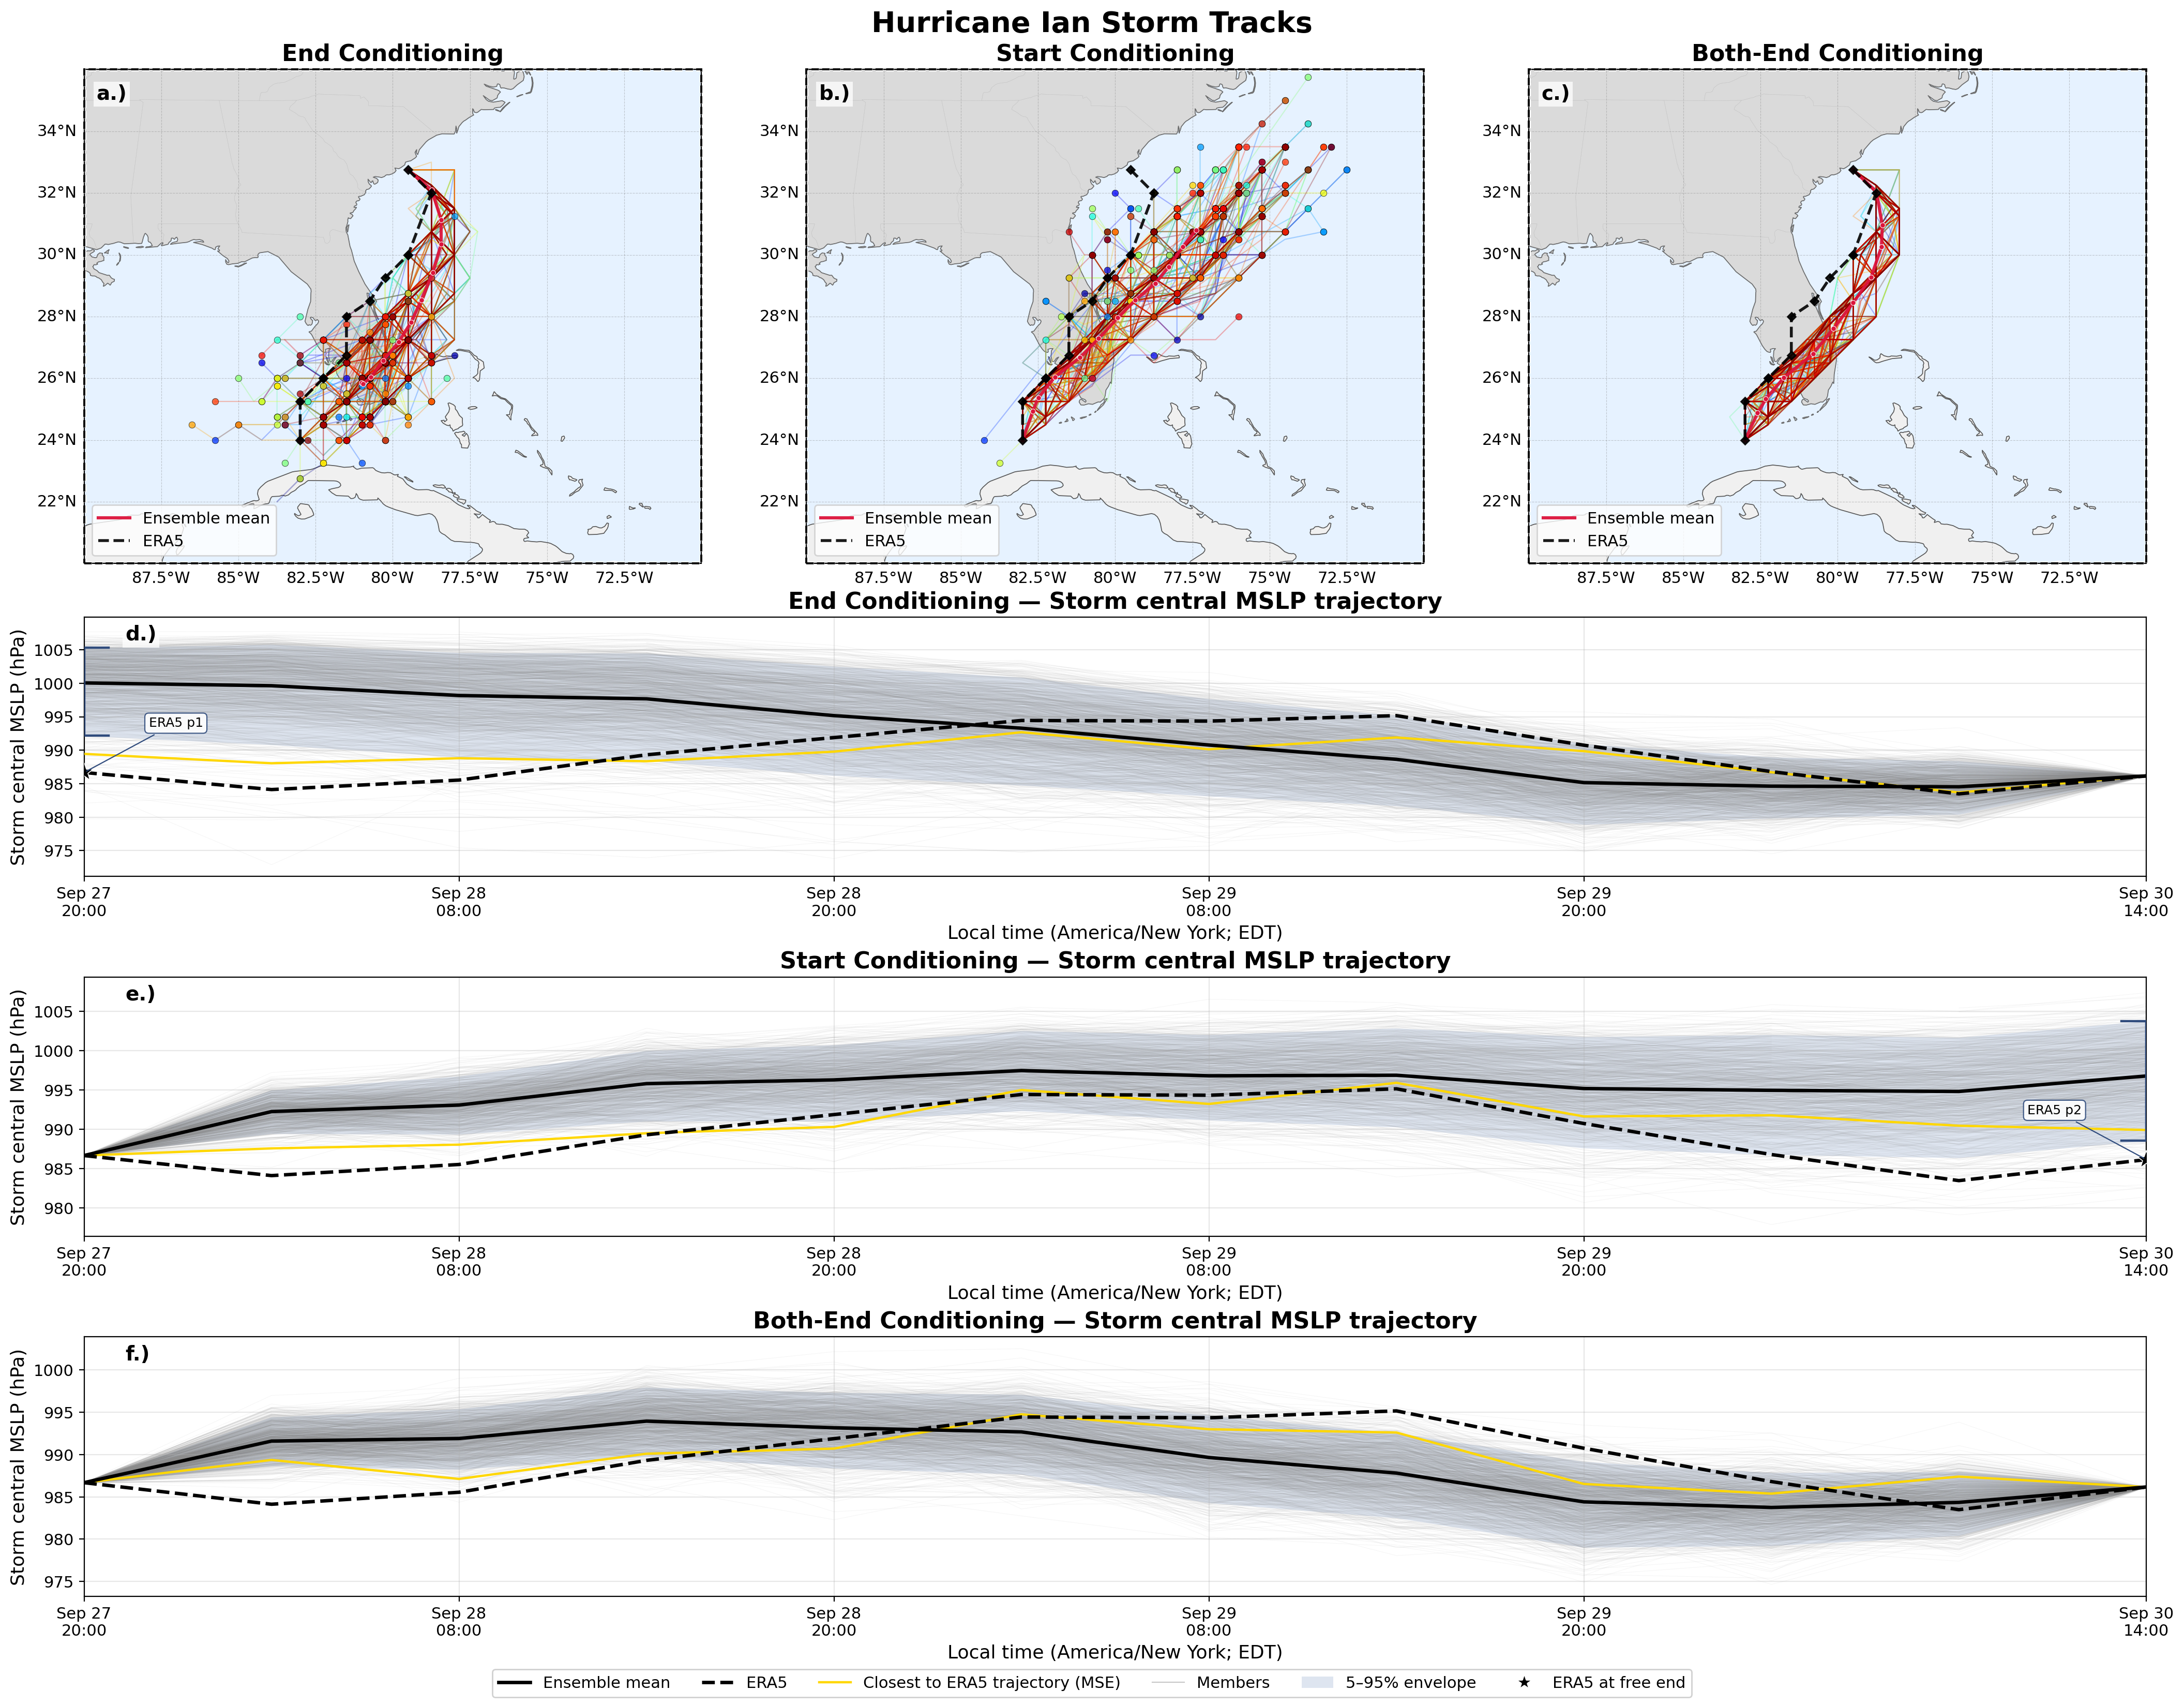
\includegraphics[width=0.82\textwidth]{ian_tc_tracks.png}
\caption{Hurricane Ian tracks and central-pressure trajectories for 1000-member ensembles under end (a,d), start (b,e), and both-end (c,f) conditioning. (a--c) Storm-center tracks connect 6-hourly TempestExtremes fixes, effectively resolved at the native HPX64 ($\sim$100~km) scale; the $0.25^{\circ}$ regridding used for tracking adds no finer-scale information. The angularity is a discrete-sampling artifact, most pronounced where the pressure minimum is weak or diffuse, and does not reflect physical track variability. (d--f) Resolved storm central pressure for individual members (gray), ensemble mean (solid black), ERA5 (dashed black), and minimum-MSE member (gold). Blue whiskers at the free-end margin in (d,e) denote the 5th--95th percentile envelope, annotated with ERA5's percentile among analyzable members: 1.0 at the end-conditioned free end and 1.8 at the start-conditioned free end. Both-end conditioning (c,f) pins both boundaries and carries no free end.}
\label{fig:ian_tc_tracks}
\end{figure}

% Figures S2-S5 carry the four hurricane track and intensity regressions.
% All four share a layout, so they share the 0.82\textwidth sizing note above:
% h/w is 0.79-0.80 here against ian_tc_tracks.png's 0.78.
\begin{figure}
\centering
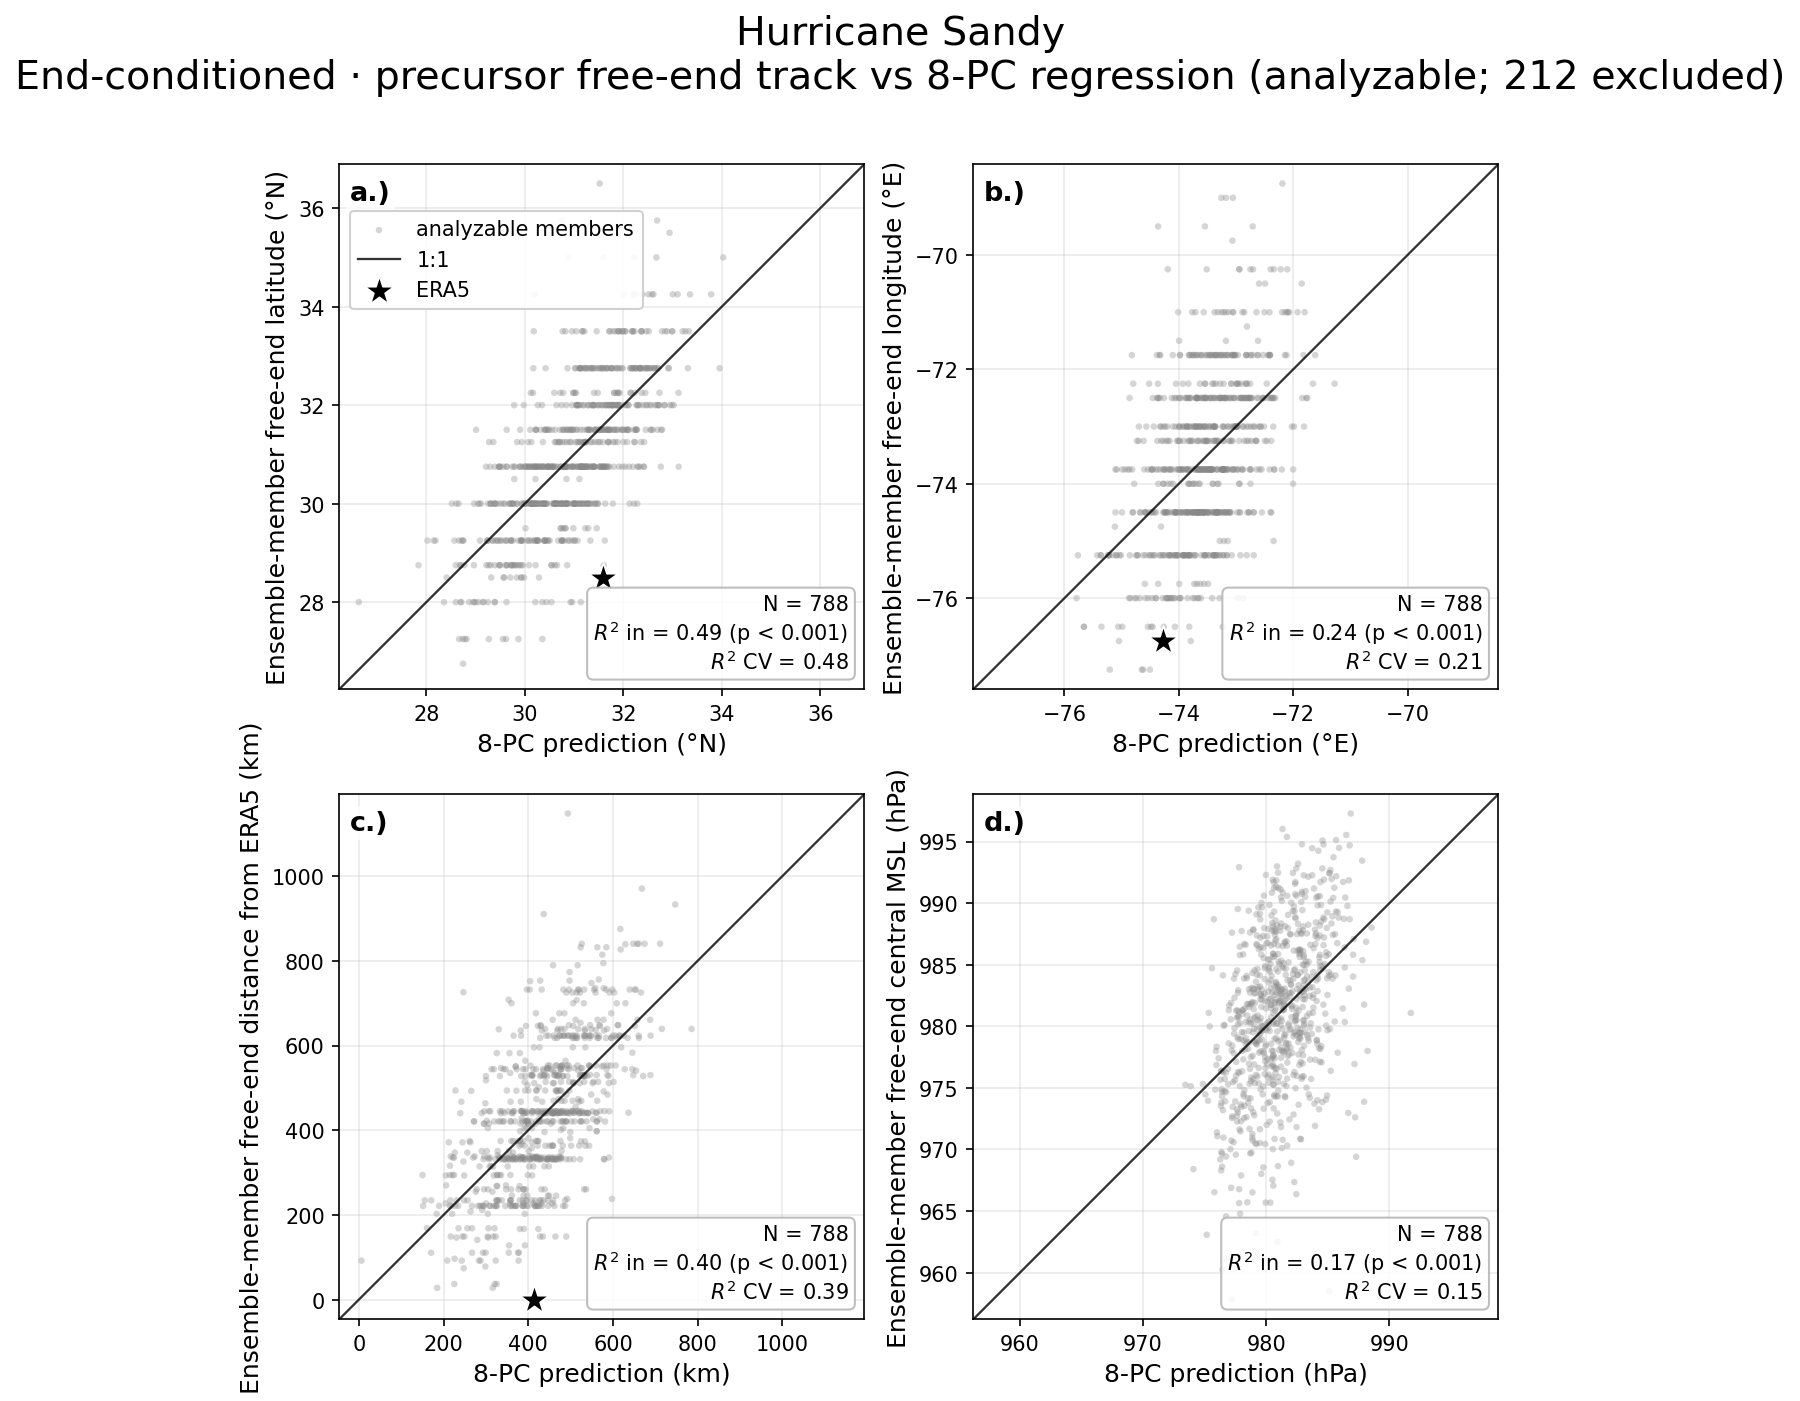
\includegraphics[width=0.82\textwidth]{sandy_track_regression_end.png}
\caption{Predicted versus ensemble-member free-end storm properties for the end-conditioned Superstorm Sandy ensemble ($N=788$ analyzable members; 212 excluded) at the precursor boundary (October 27, 2012, 06:00 UTC): (a) latitude, (b) longitude, (c) great-circle distance from the ERA5 fix, and (d) central MSLP. Predictions are from ordinary least-squares regressions on the leading eight principal components of the free-end $z_{500}$ field ($100^{\circ}$--$30^{\circ}$~W, $25^{\circ}$--$75^{\circ}$~N); insets report in-sample and 10-fold cross-validated $R^2$. The star marks ERA5 evaluated at its observed $z_{500}$ state. Panel (a) is the source of the 48\% variance explained quoted in Section~3.2.}
\label{fig:sandy_track_regression_end}
\end{figure}

\begin{figure}
\centering
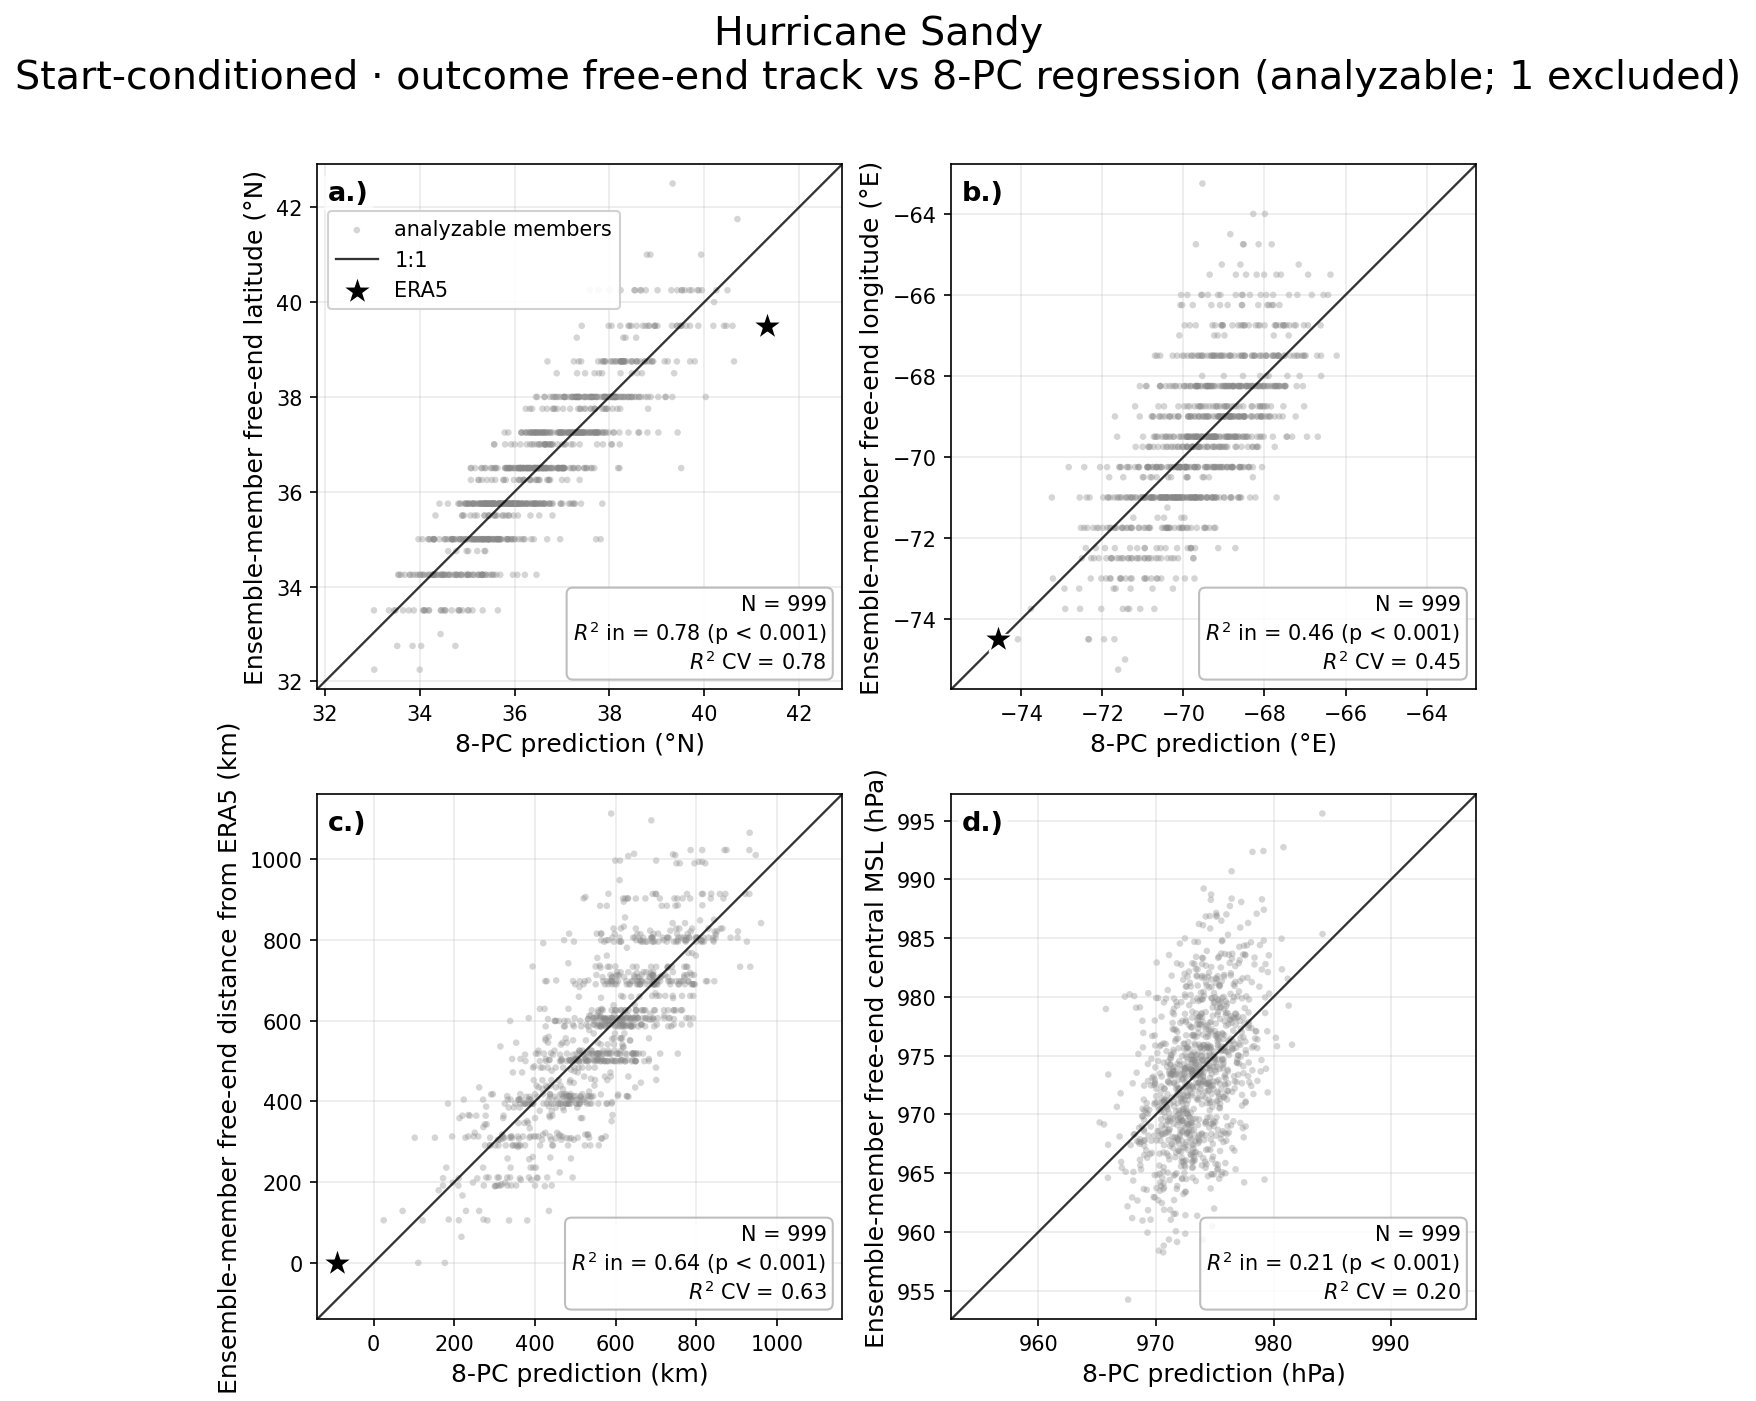
\includegraphics[width=0.82\textwidth]{sandy_track_regression_start.png}
\caption{Predicted versus ensemble-member free-end storm properties for the start-conditioned Superstorm Sandy ensemble ($N=984$ analyzable members; 16 excluded) at the outcome boundary (October 30, 2012, 00:00 UTC), as in Figure~S2: (a) latitude, (b) longitude, (c) great-circle distance from the ERA5 fix, and (d) central MSLP. Predictions use ordinary least-squares regressions on the leading eight principal components of the free-end $z_{500}$ field ($100^{\circ}$--$30^{\circ}$~W, $25^{\circ}$--$75^{\circ}$~N); insets report in-sample and 10-fold cross-validated $R^2$. The star marks ERA5 evaluated at its observed $z_{500}$ state. Panel (a) is the source of the 79\% variance explained quoted in Section~3.2.}
\label{fig:sandy_track_regression_start}
\end{figure}

\begin{figure}
\centering
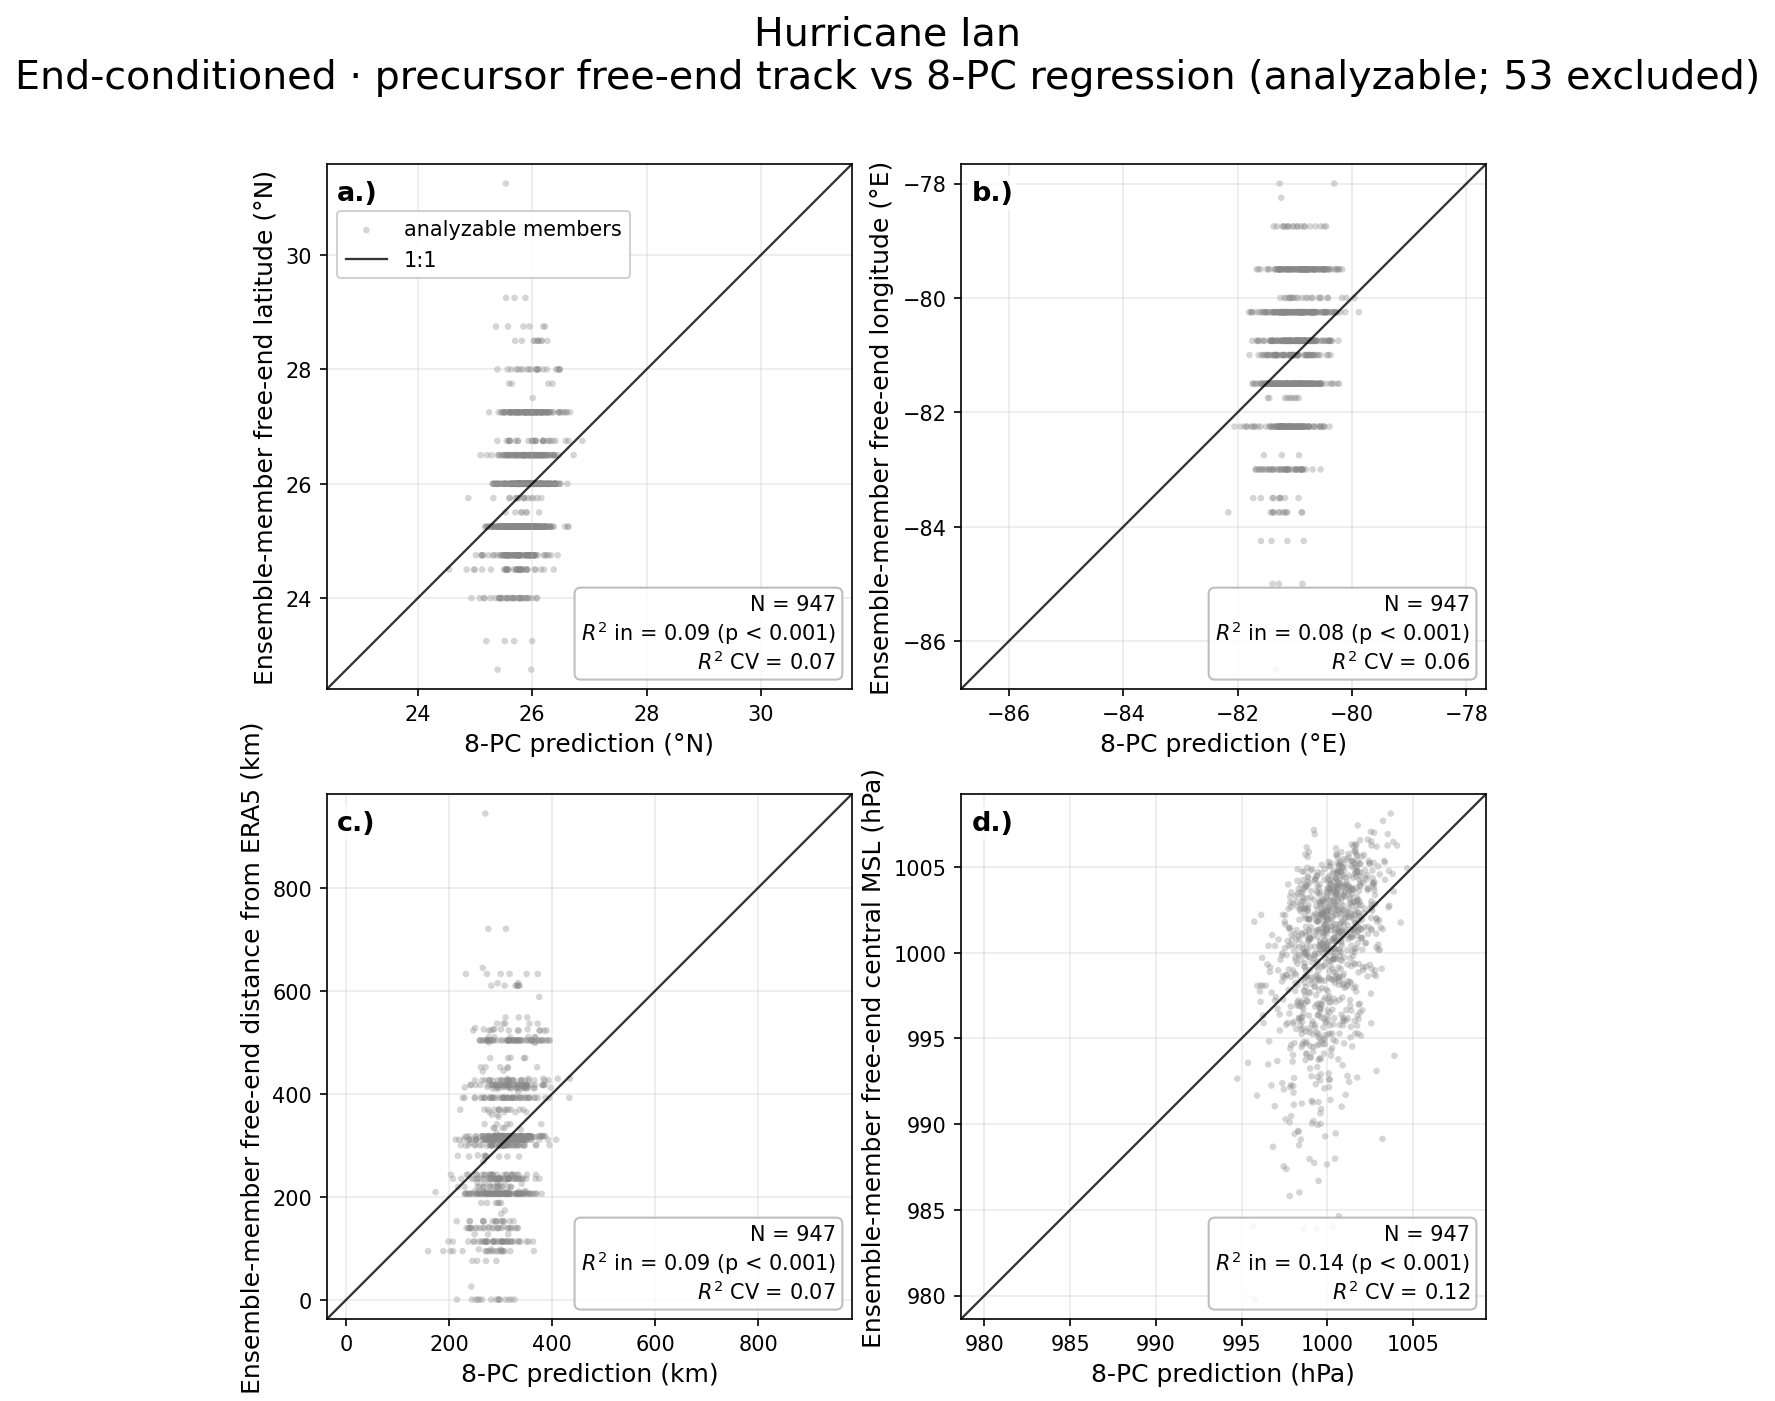
\includegraphics[width=0.82\textwidth]{ian_track_regression_end.png}
\caption{Predicted versus ensemble-member free-end storm properties for the end-conditioned Hurricane Ian ensemble ($N=947$ analyzable members; 53 excluded) at the precursor boundary (September 28, 2022, 00:00 UTC): (a) latitude, (b) longitude, (c) great-circle distance from the ERA5 fix, and (d) central MSLP. Predictions are from ordinary least-squares regressions on the leading eight principal components of the free-end $z_{500}$ field ($110^{\circ}$--$50^{\circ}$~W, $15^{\circ}$--$50^{\circ}$~N); insets report in-sample and 10-fold cross-validated $R^2$. Panel (a) is the source of the $\sim$7\% variance explained quoted in Section~3.3.}
\label{fig:ian_track_regression_end}
\end{figure}

\begin{figure}
\centering
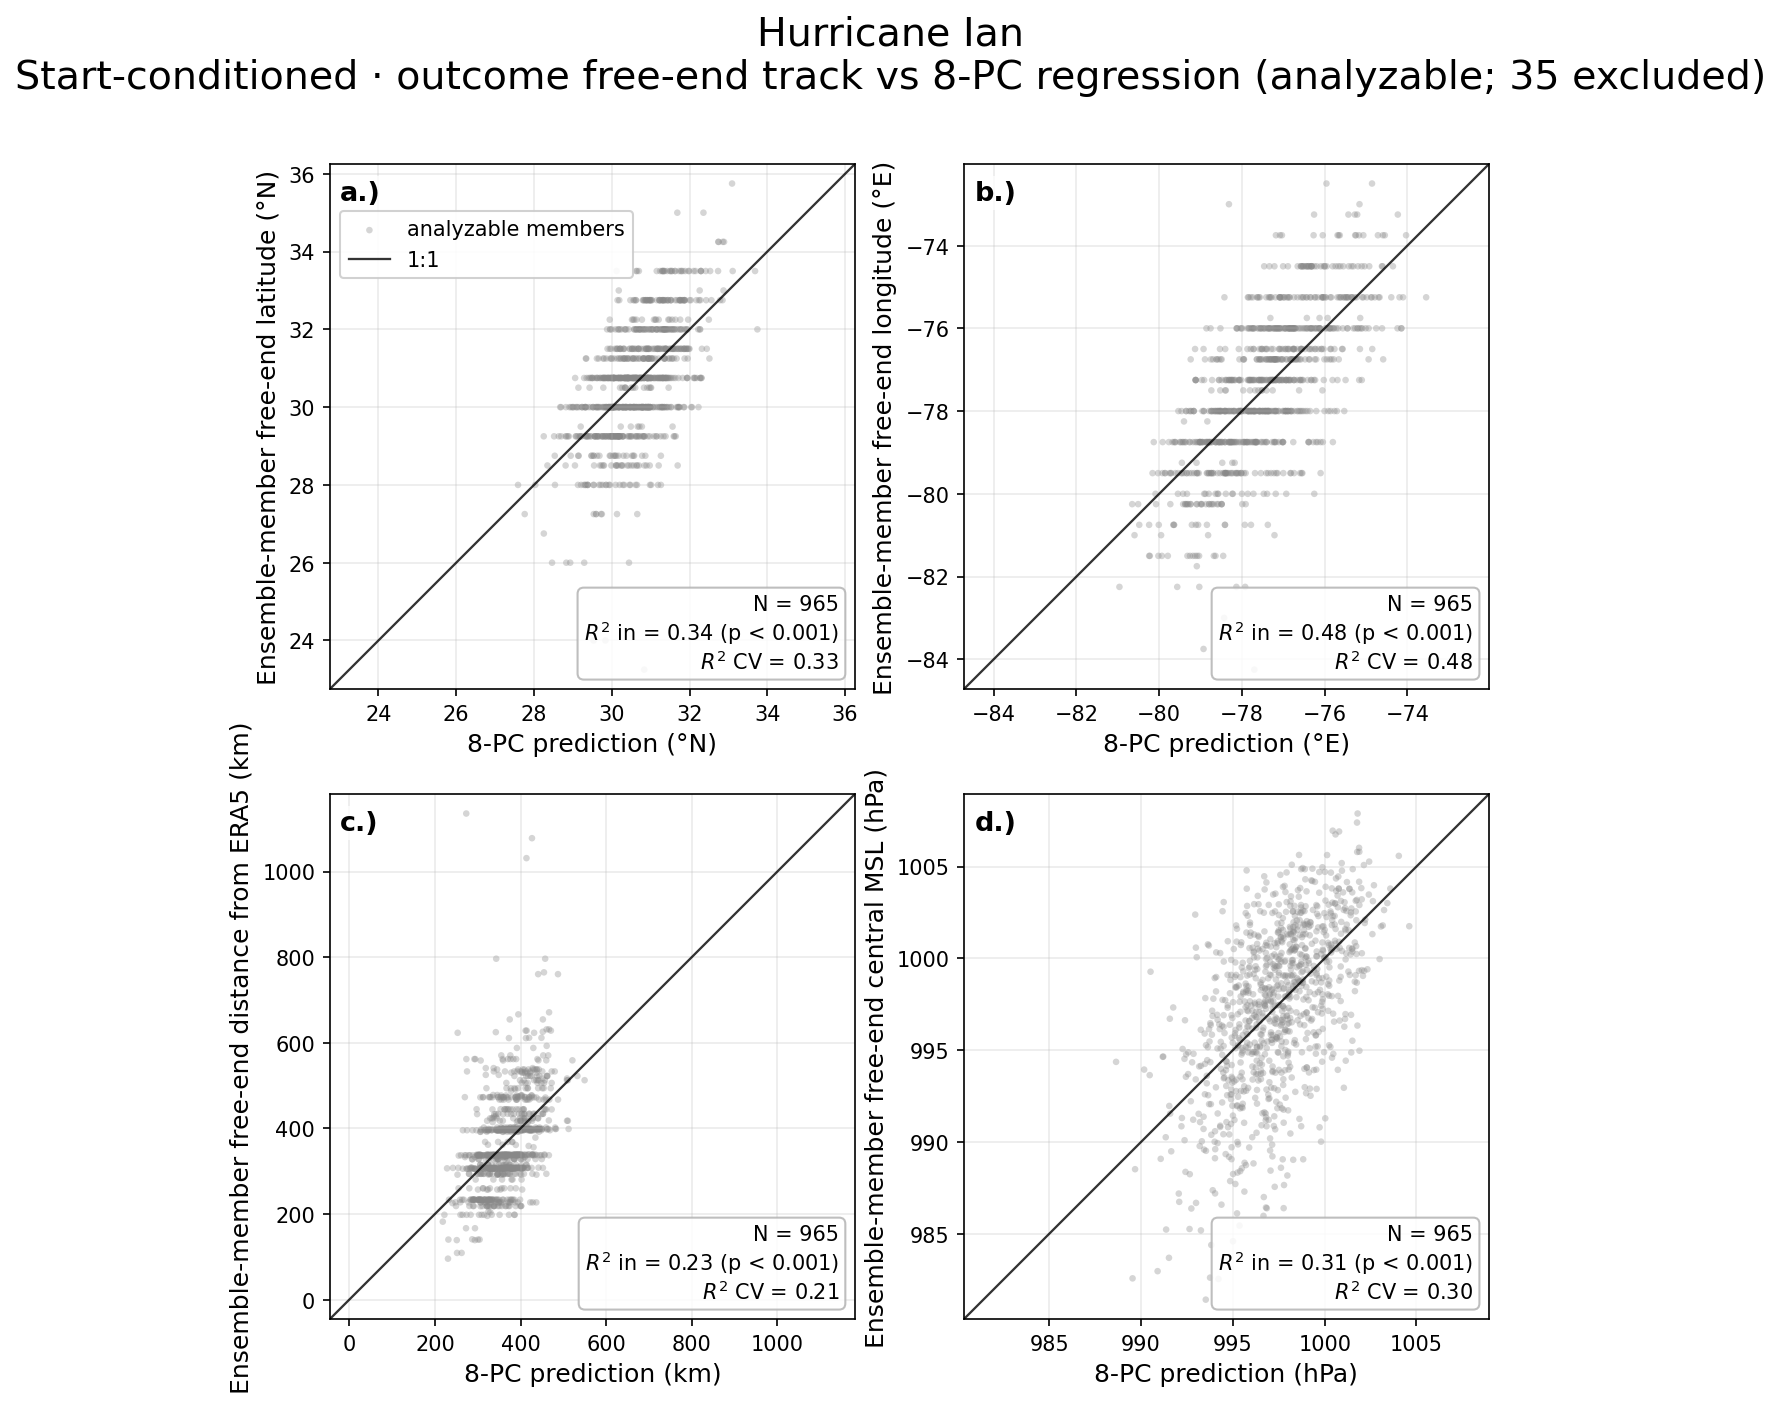
\includegraphics[width=0.82\textwidth]{ian_track_regression_start.png}
\caption{As in Figure~S4, but for the start-conditioned Hurricane Ian ensemble ($N=757$ analyzable members; 243 excluded) at the outcome boundary (September 30, 2022, 18:00 UTC). Panels (b), (a), and (c) are the sources of the 52\%, 40\%, and 20\% variance explained quoted in Section~3.3. Read against Figure~S4 (same case, domain, and regressions under reversed conditioning), this pair illustrates the start-versus-end asymmetry described in Section~3.3.}
\label{fig:ian_track_regression_start}
\end{figure}

% Figures S6-S11 are the spread/RMSE/CRPS verification battery, one per
% (case, variable) pair. Each PNG is already a complete five-panel figure, so
% they are not composed further: merging a case's two variables into one float
% would duplicate the (a)-(e) panel letters. These are taller than the
% regression figures (h/w = 0.90 against 0.79-0.80), so 0.72\textwidth here
% gives the same rendered height that 0.82\textwidth gives them.
\begin{figure}
\centering
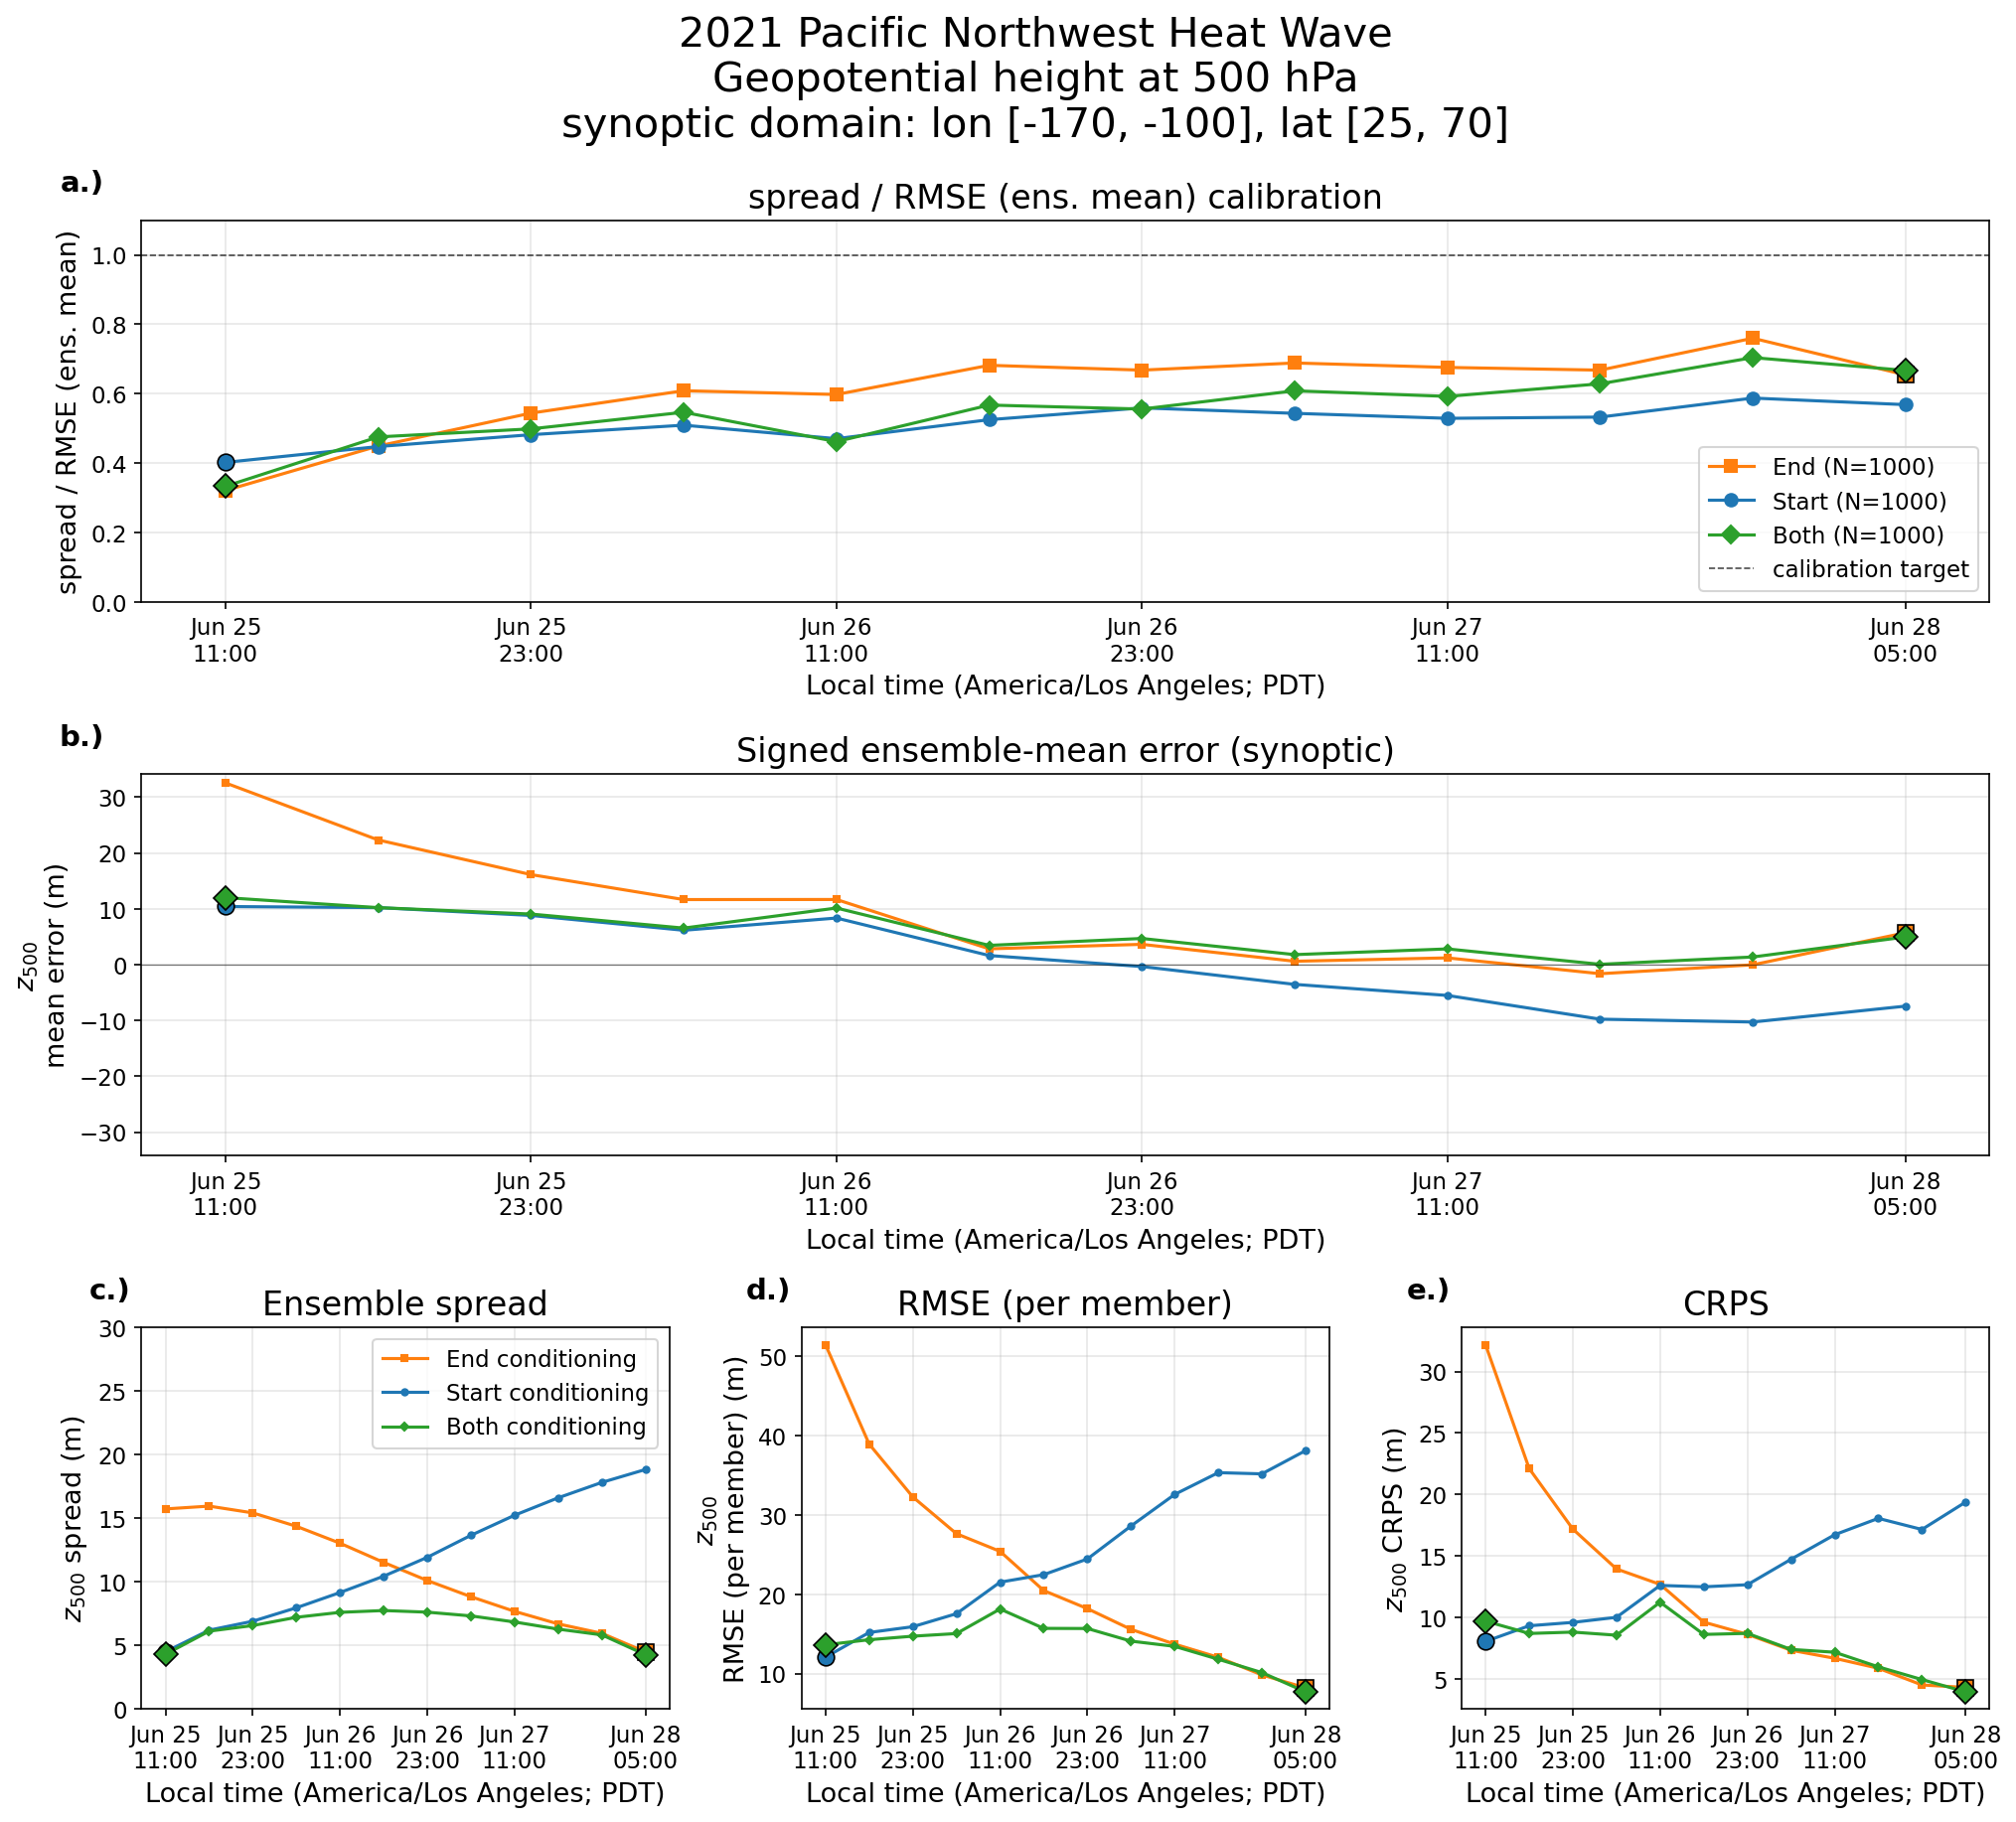
\includegraphics[width=0.72\textwidth]{spread_rmse_crps_pnw_heatwave_z500.png}
\caption{Ensemble spread, ensemble-mean error, and probabilistic skill against ERA5 as a function of lead time for the 2021 Pacific Northwest heatwave $z_{500}$ field over the synoptic domain ($170^{\circ}$--$100^{\circ}$~W, $25^{\circ}$--$70^{\circ}$~N), across all three conditioning modes ($N = 1000$ each). (a) Ratio of ensemble spread to ensemble-mean RMSE (dashed horizontal line at unity denotes statistical consistency; values below unity indicate under-dispersion). (b) Signed ensemble-mean error. (c) Domain-mean ensemble spread (Equation~S7). (d) Per-member RMSE. (e) Continuous ranked probability score (CRPS). Enlarged markers denote pinned boundaries (start, end, or both). Quantities are domain-averaged over native equal-area HEALPix pixels without latitude weighting. Free-end spreads in (c)---15.7~m end-conditioned and 18.8~m start-conditioned---form the 0.84 ratio reported in Text~S4.}
\label{fig:spread_rmse_crps_pnw_heatwave_z500}
\end{figure}

\begin{figure}
\centering
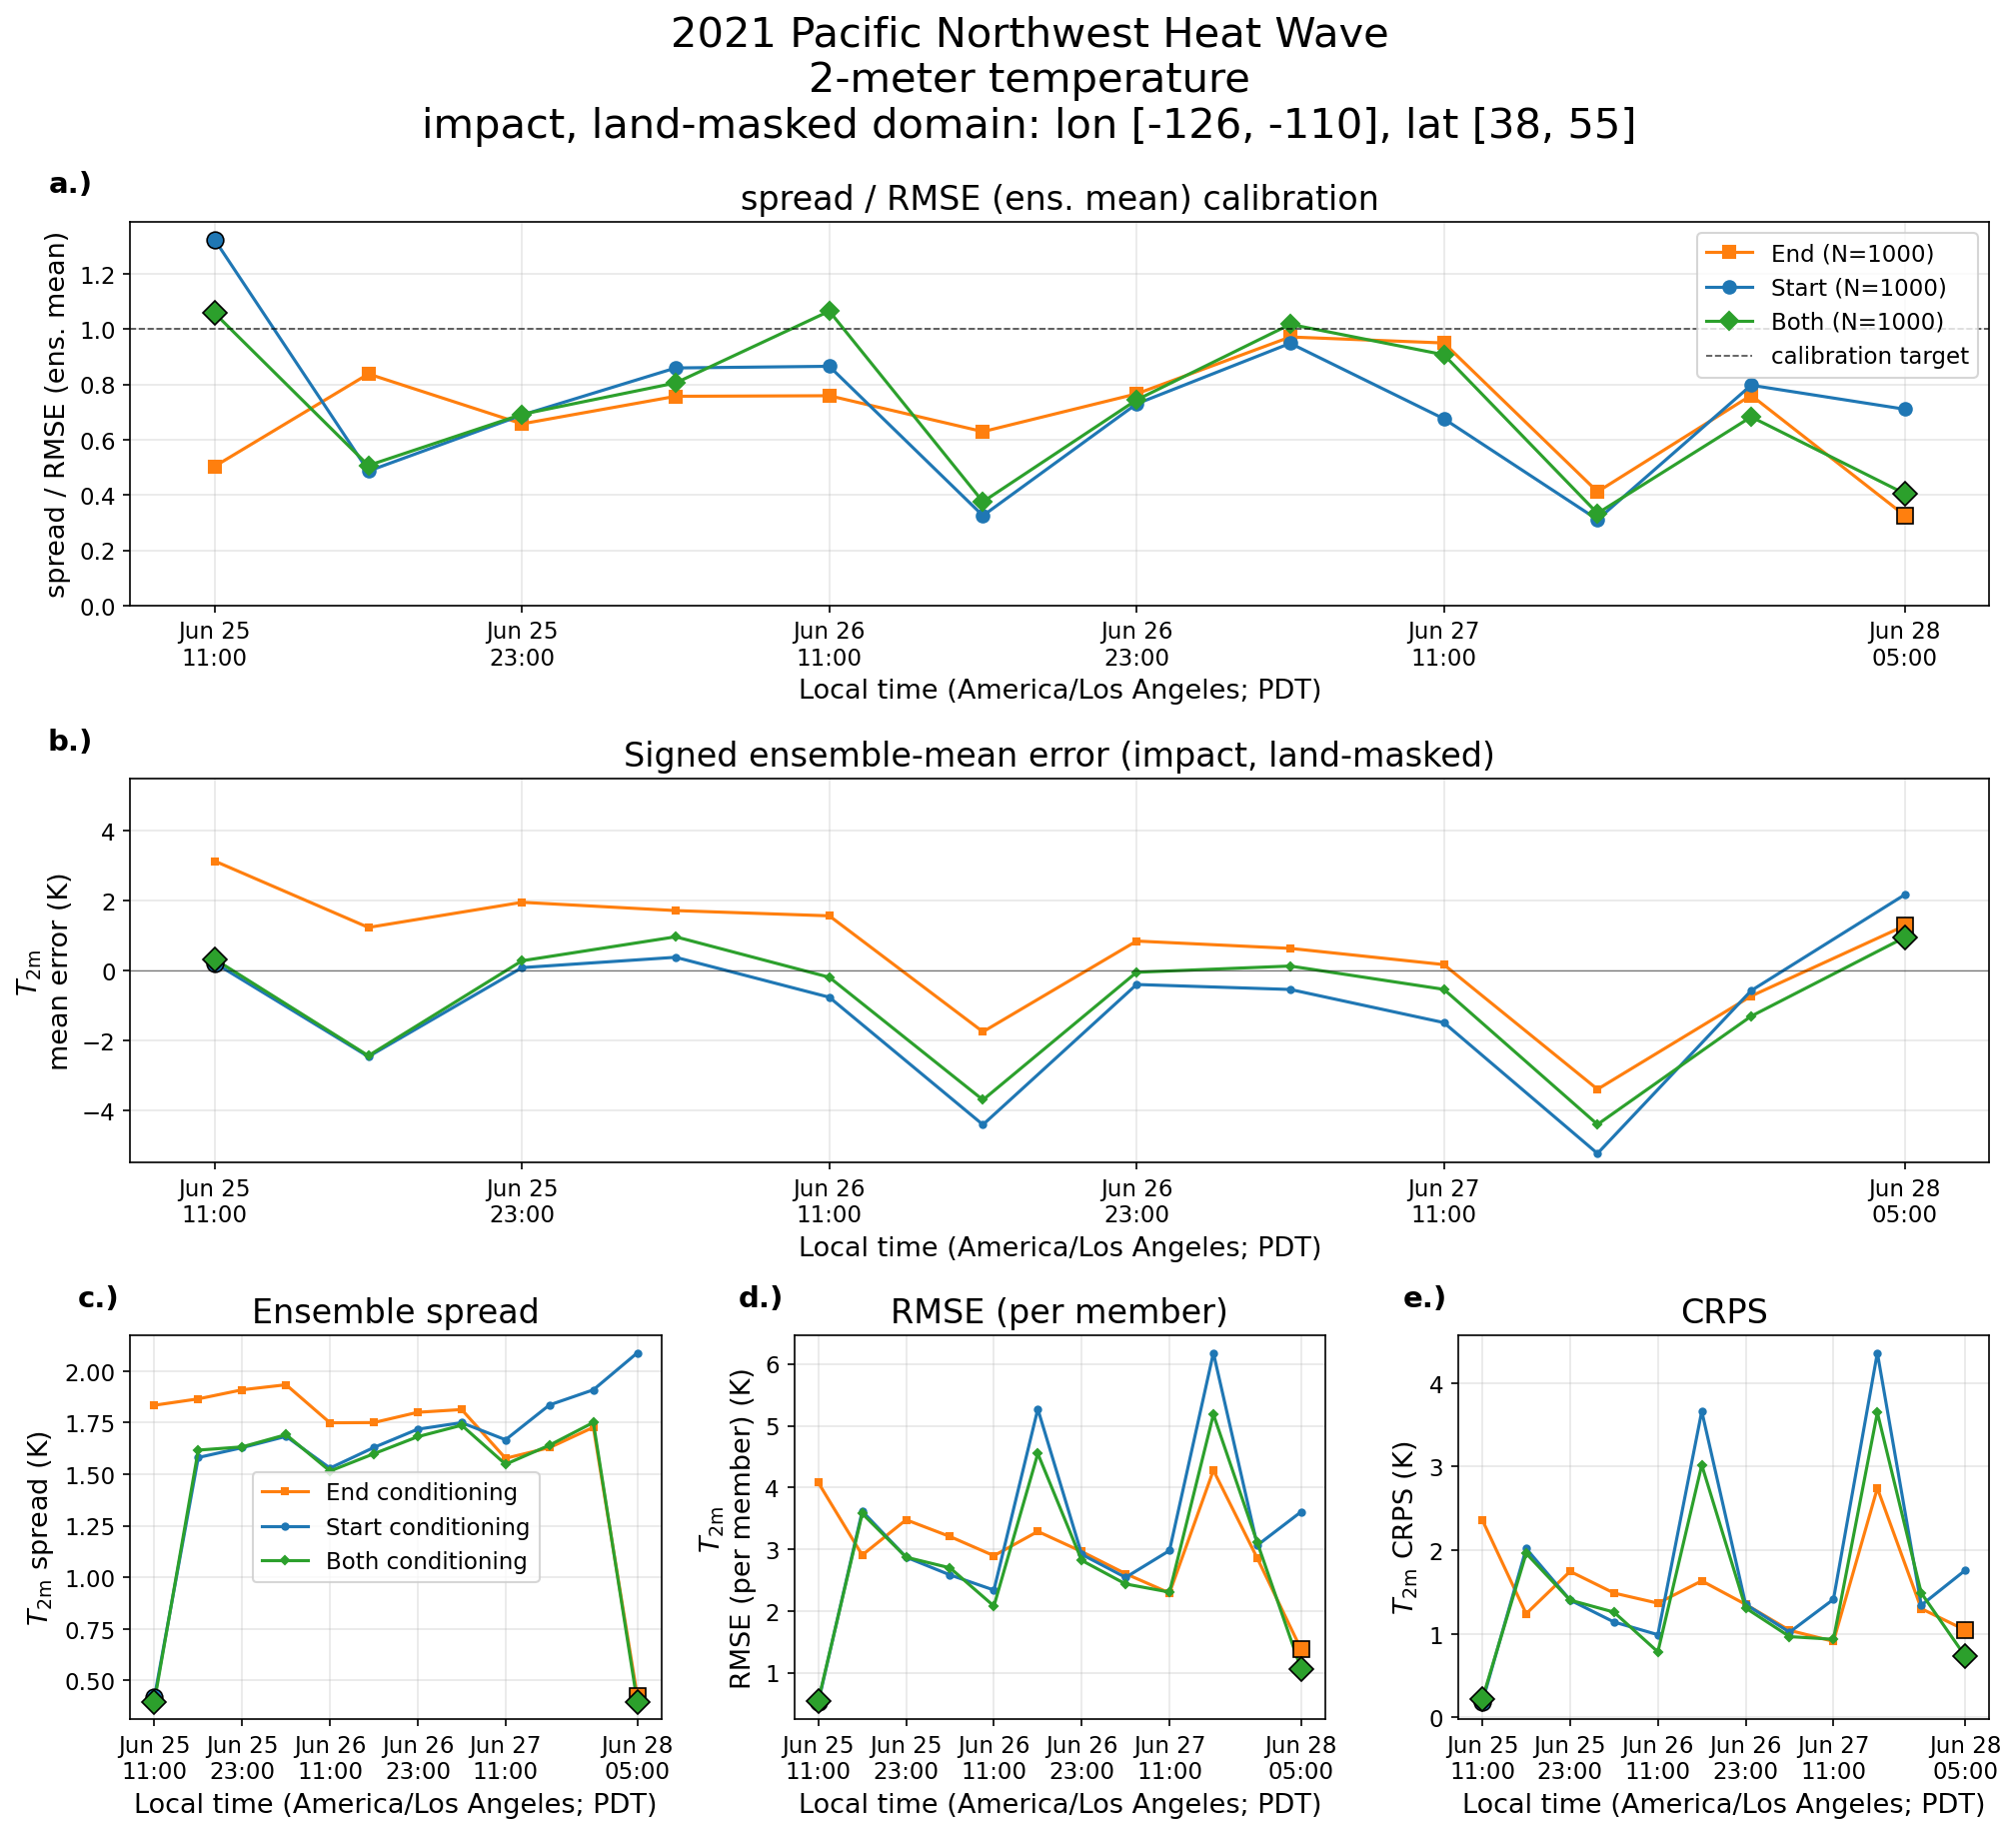
\includegraphics[width=0.72\textwidth]{spread_rmse_crps_pnw_heatwave_t2m.png}
\caption{As in Figure~S6, but for 2-meter temperature over land pixels of the impact domain ($126^{\circ}$--$110^{\circ}$~W, $38^{\circ}$--$55^{\circ}$~N), using the land mask defined in Section~3.1. Ocean pixels are excluded because they track prescribed, member-identical sea surface temperatures. Unlike the $z_{500}$ and MSLP fields of Figures~S6 and S8--S11, the spread-to-error ratio in (a) reaches and exceeds unity across several frames, demonstrating that under-dispersion is not universal across all variables.}
\label{fig:spread_rmse_crps_pnw_heatwave_t2m}
\end{figure}

\begin{figure}
\centering
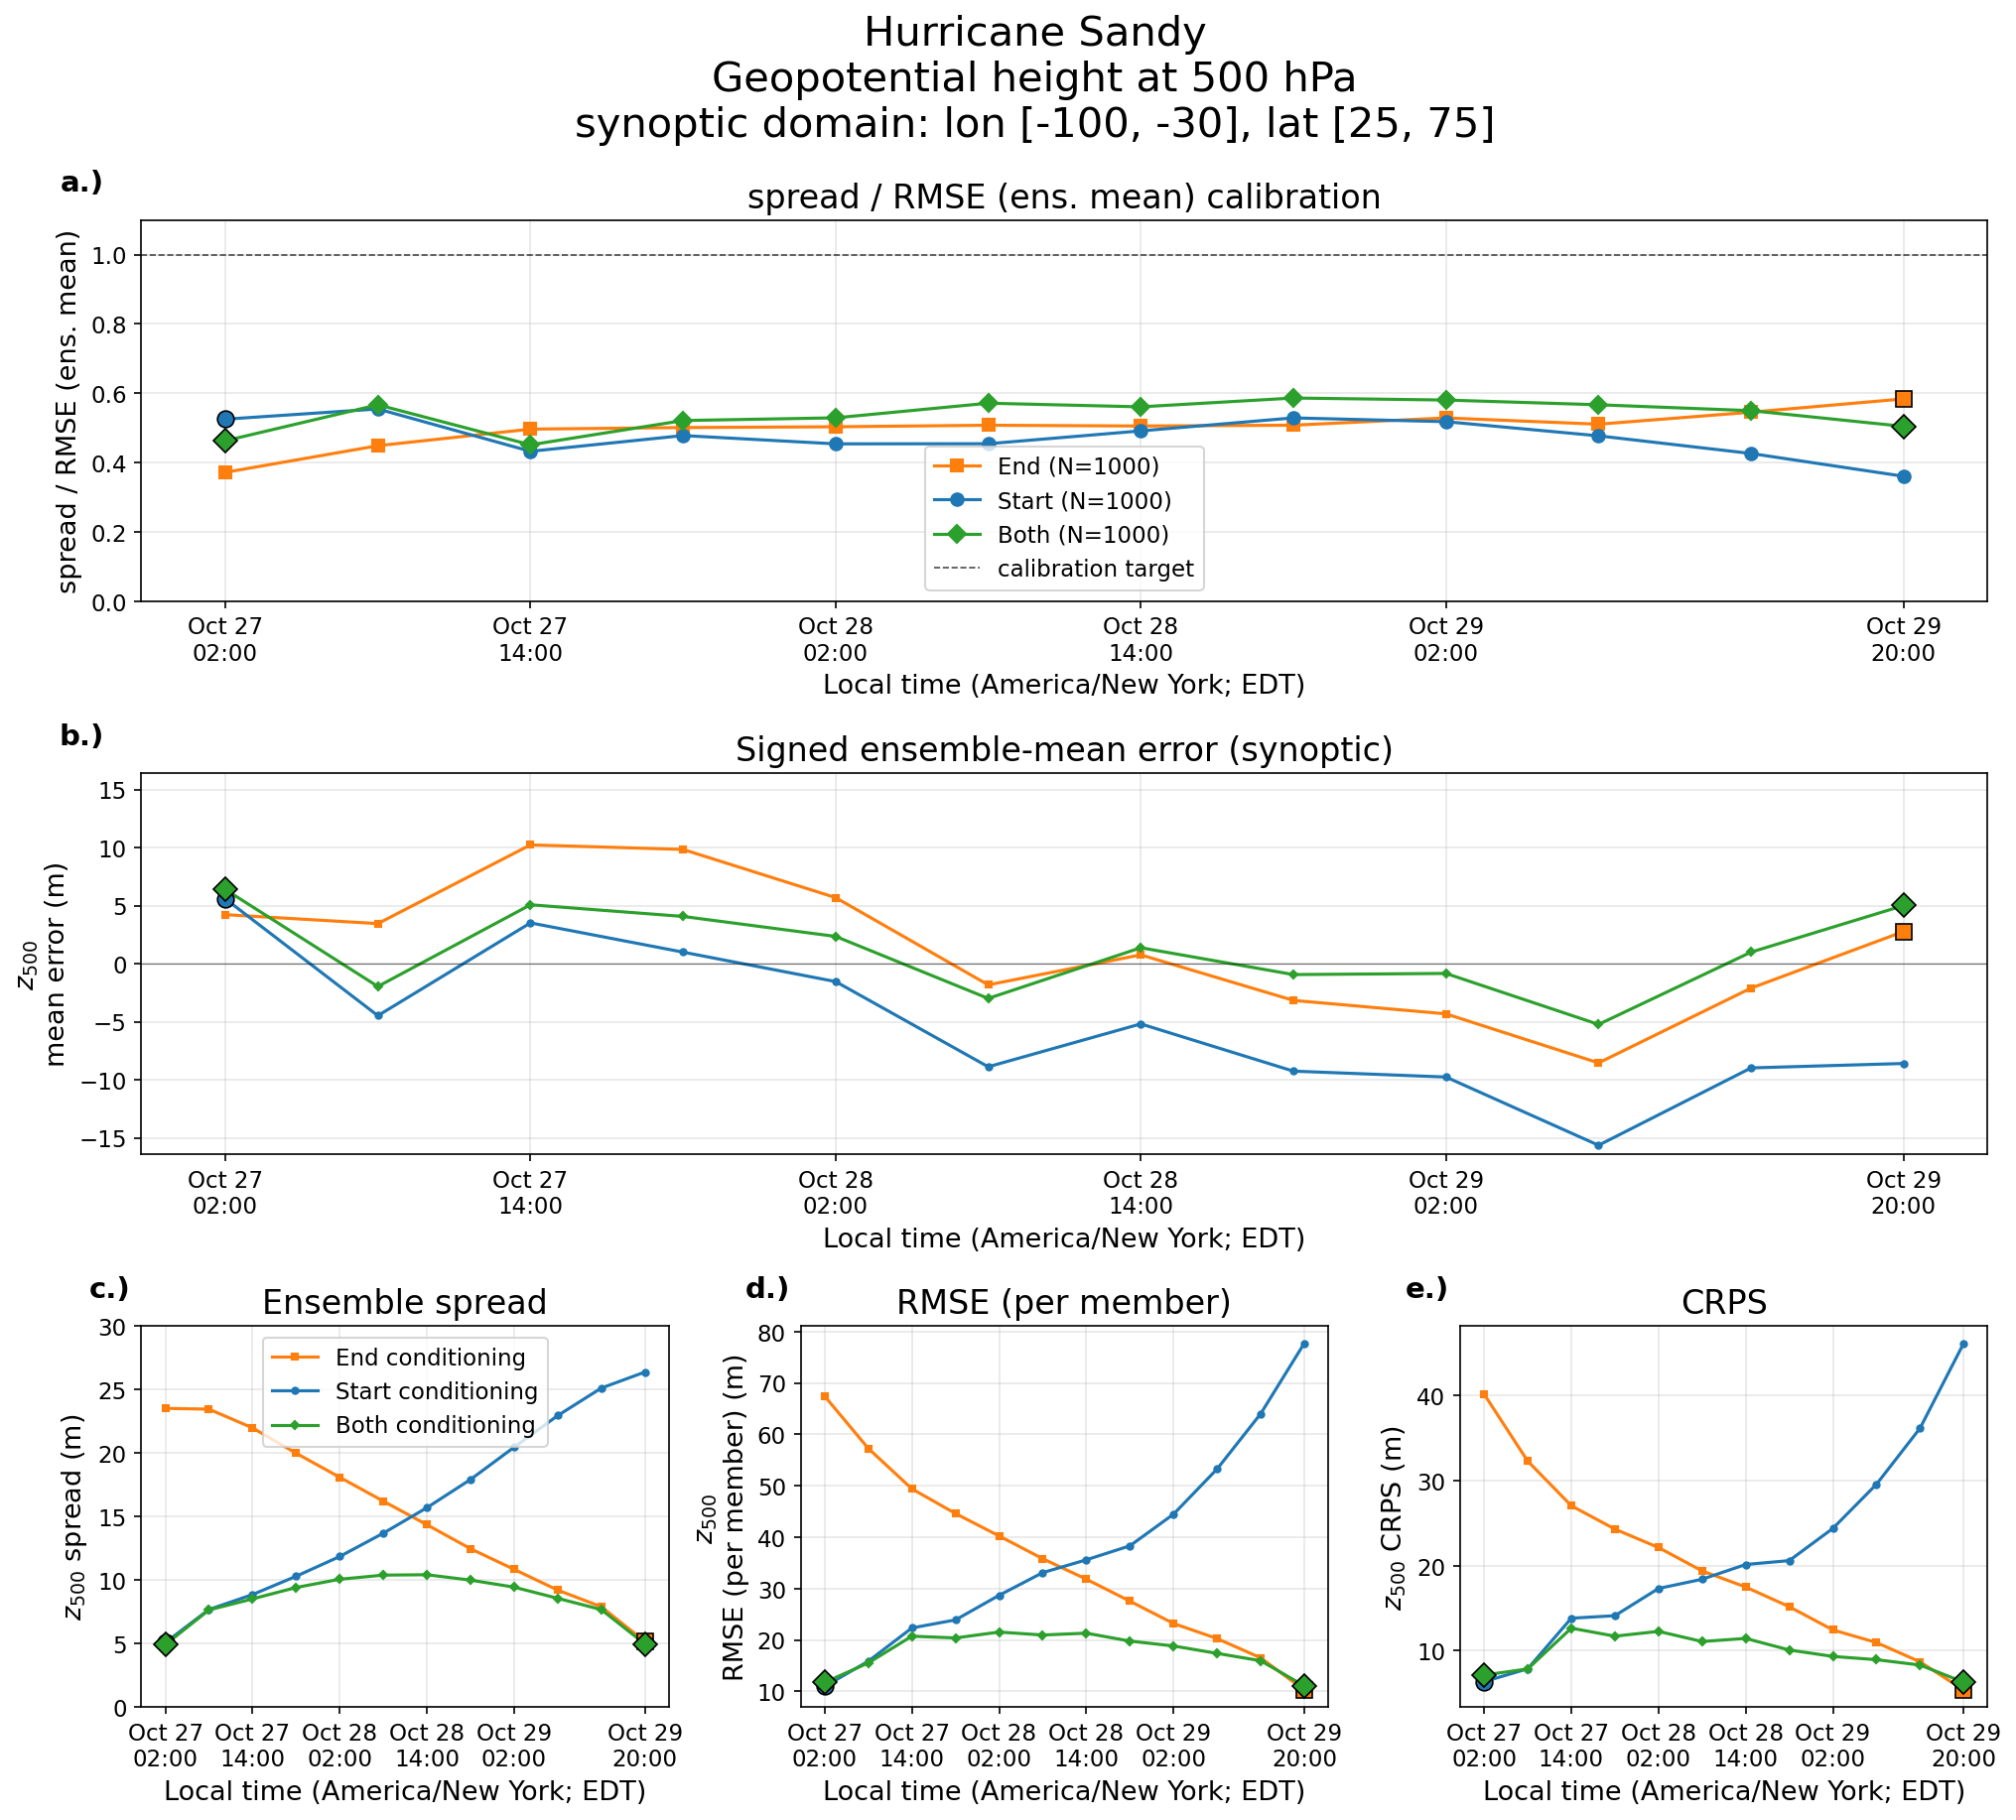
\includegraphics[width=0.72\textwidth]{spread_rmse_crps_sandy_z500.png}
\caption{As in Figure~S6, but for Superstorm Sandy $z_{500}$ over its synoptic domain ($100^{\circ}$--$30^{\circ}$~W, $25^{\circ}$--$75^{\circ}$~N), matching the domain used for EOF analysis and Text~S4. Free-end spreads in (c)---23.5~m end-conditioned and 26.4~m start-conditioned---form the 0.89 ratio reported in Text~S4.}
\label{fig:spread_rmse_crps_sandy_z500}
\end{figure}

\begin{figure}
\centering
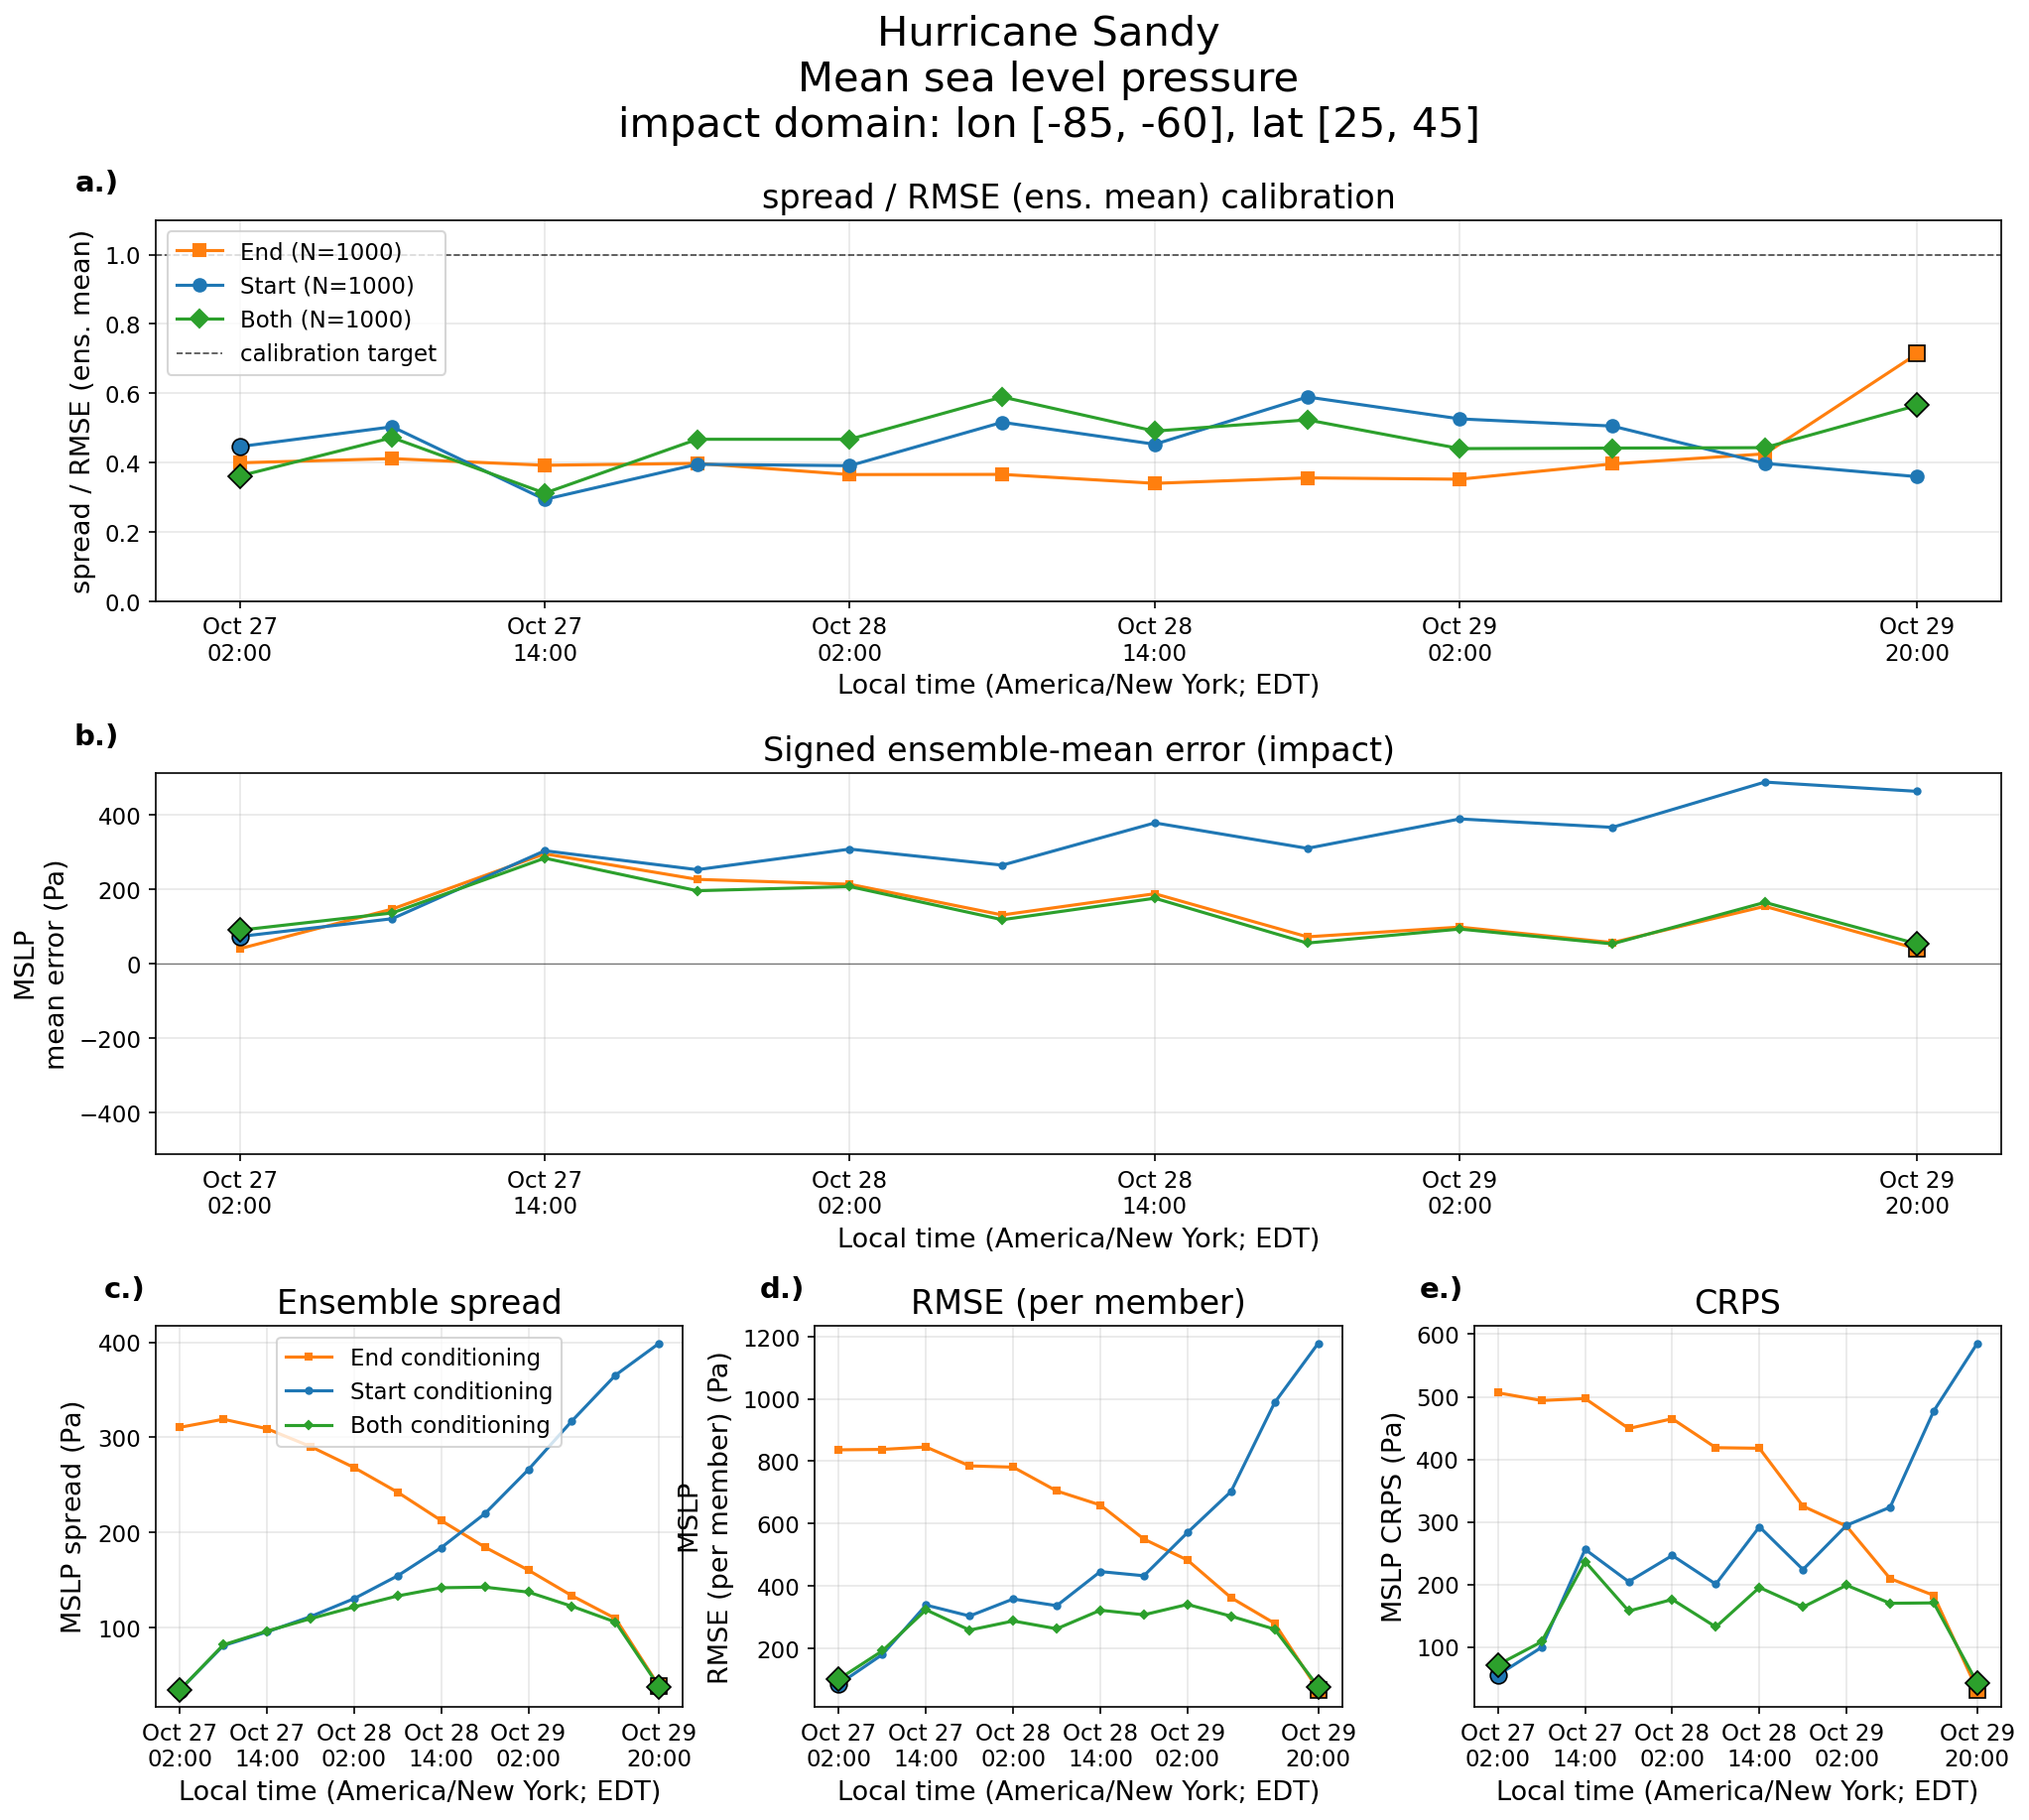
\includegraphics[width=0.72\textwidth]{spread_rmse_crps_sandy_msl.png}
\caption{As in Figure~S8, but for mean sea level pressure (MSLP) over the cyclone impact domain ($85^{\circ}$--$60^{\circ}$~W, $25^{\circ}$--$45^{\circ}$~N). The end-to-start free-end spread ratio in (c) is 0.78 for MSLP over this localized domain, distinct from the synoptic $z_{500}$ spread ratios defined in Text~S4.}
\label{fig:spread_rmse_crps_sandy_msl}
\end{figure}

\begin{figure}
\centering
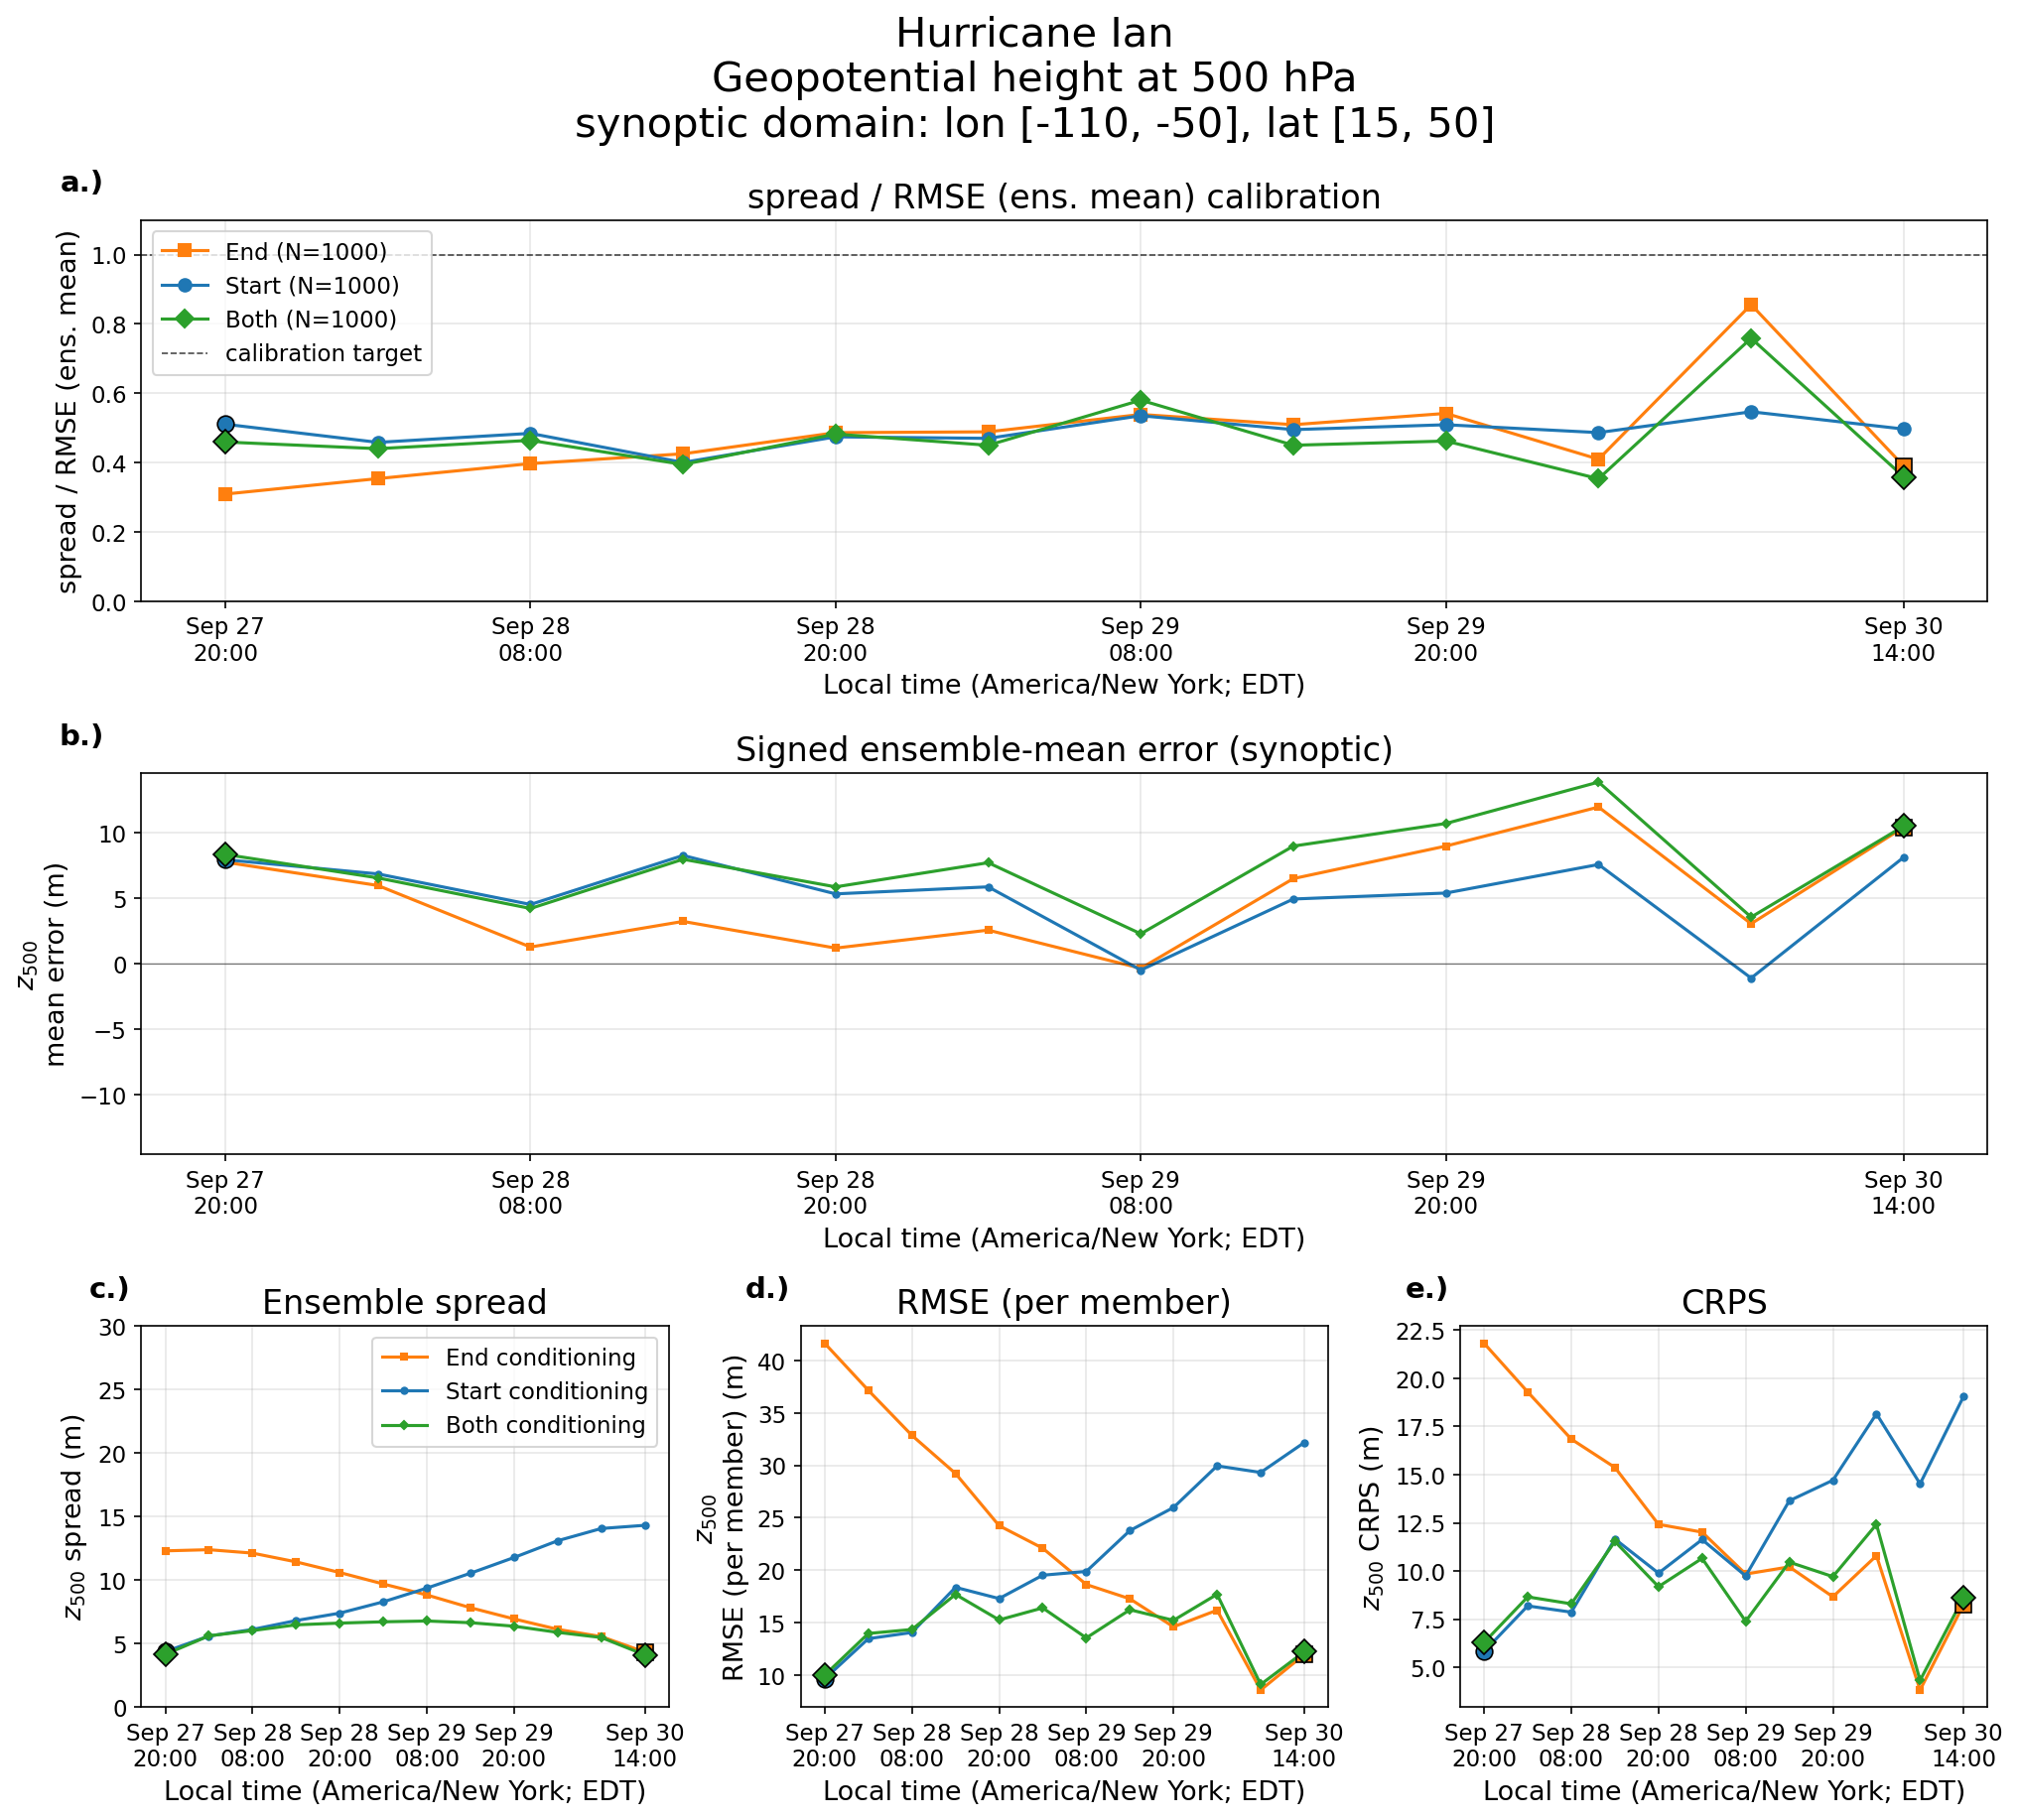
\includegraphics[width=0.72\textwidth]{spread_rmse_crps_ian_z500.png}
\caption{As in Figure~S6, but for Hurricane Ian $z_{500}$ over its synoptic domain ($110^{\circ}$--$50^{\circ}$~W, $15^{\circ}$--$50^{\circ}$~N). Free-end spreads in (c)---12.3~m end-conditioned and 14.3~m start-conditioned---form the 0.86 ratio reported in Text~S4.}
\label{fig:spread_rmse_crps_ian_z500}
\end{figure}

\begin{figure}
\centering
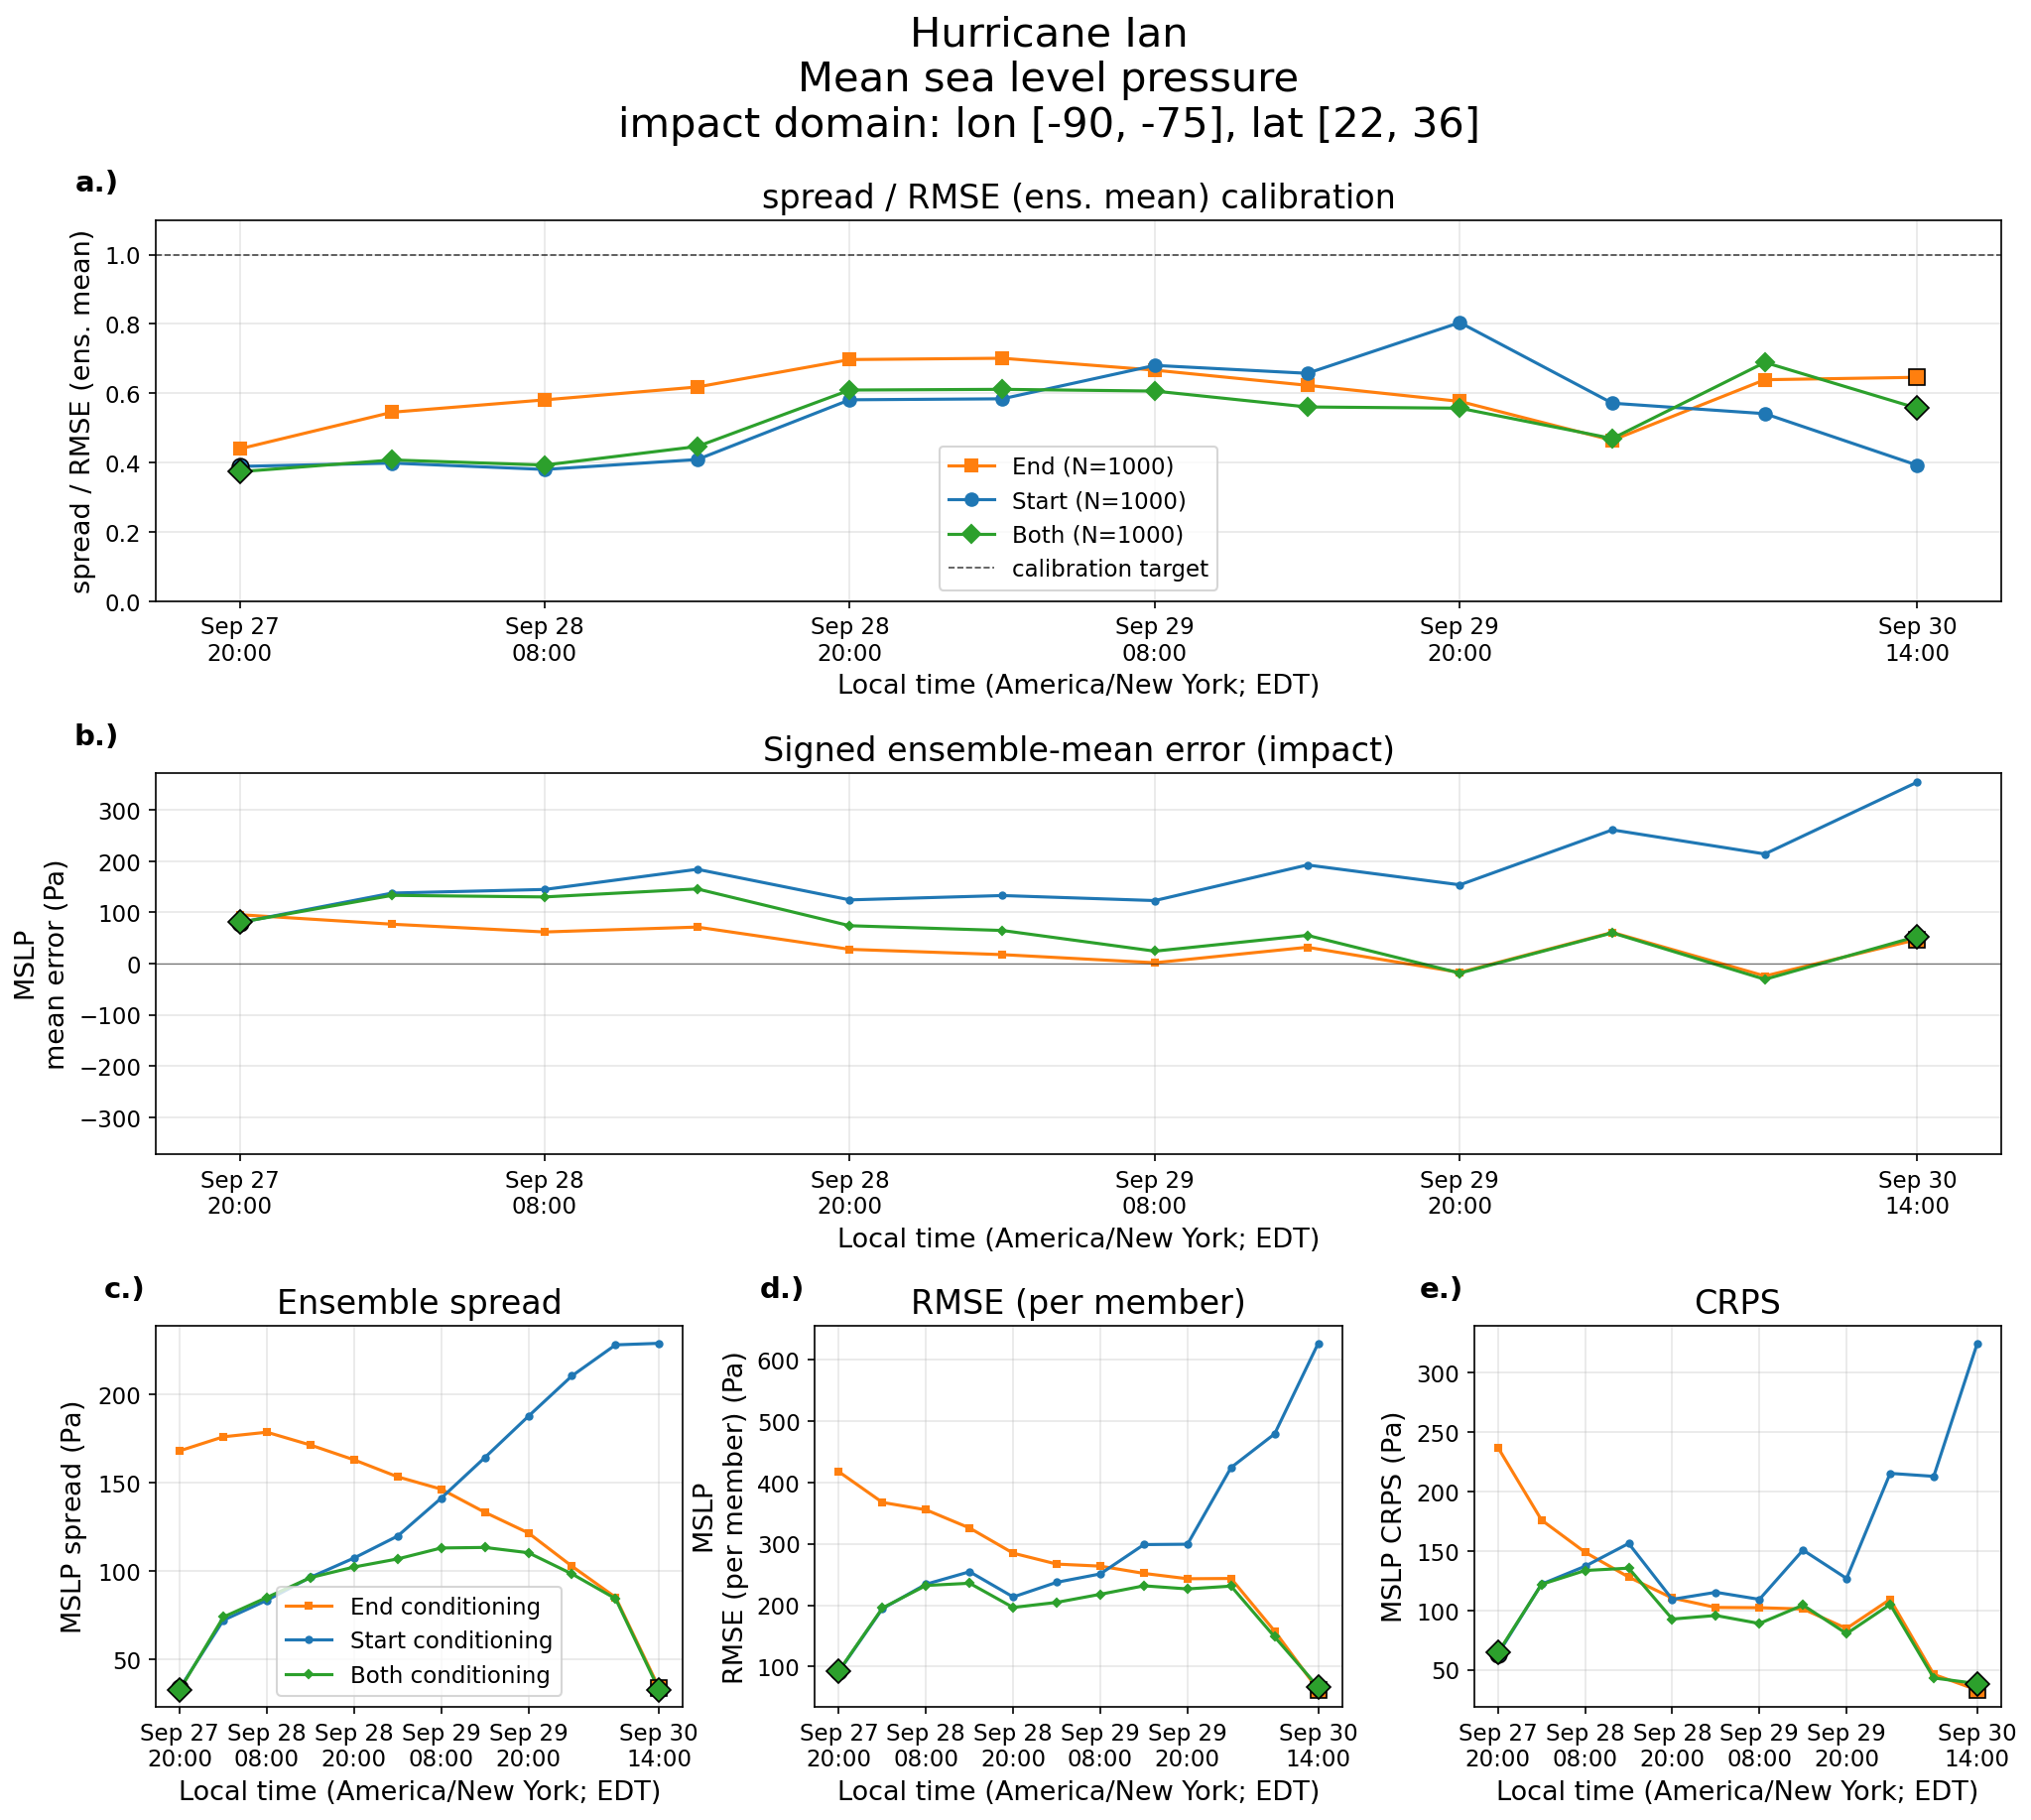
\includegraphics[width=0.72\textwidth]{spread_rmse_crps_ian_msl.png}
\caption{As in Figure~S10, but for mean sea level pressure (MSLP) over the cyclone impact domain ($90^{\circ}$--$75^{\circ}$~W, $22^{\circ}$--$36^{\circ}$~N). The end-to-start free-end spread ratio in (c) is 0.75 for MSLP over this impact domain, distinct from the synoptic $z_{500}$ ratio of Text~S4.}
\label{fig:spread_rmse_crps_ian_msl}
\end{figure}

% Figure S12 is the conditioning stress test cited from D3 of the Discussion.
% It is an EXISTENCE demonstration for the admissibility point, not a
% characterization of a boundary, so no member count or random-draw disclaimer
% belongs in the caption (PAPER_PLAN.md, parked-design amendment 2026-08-14).
% Full width because the panels are wide (h/w = 0.64 against the regression
% figures' 0.79-0.80). The caption must disclose the contrivances -- cross-period
% pair, SST clocked to start_time, frame-11 slot/field clock mismatch -- because
% the panel headers make the year jump between F10 and F11 visible to any reader.
\begin{figure}
\centering
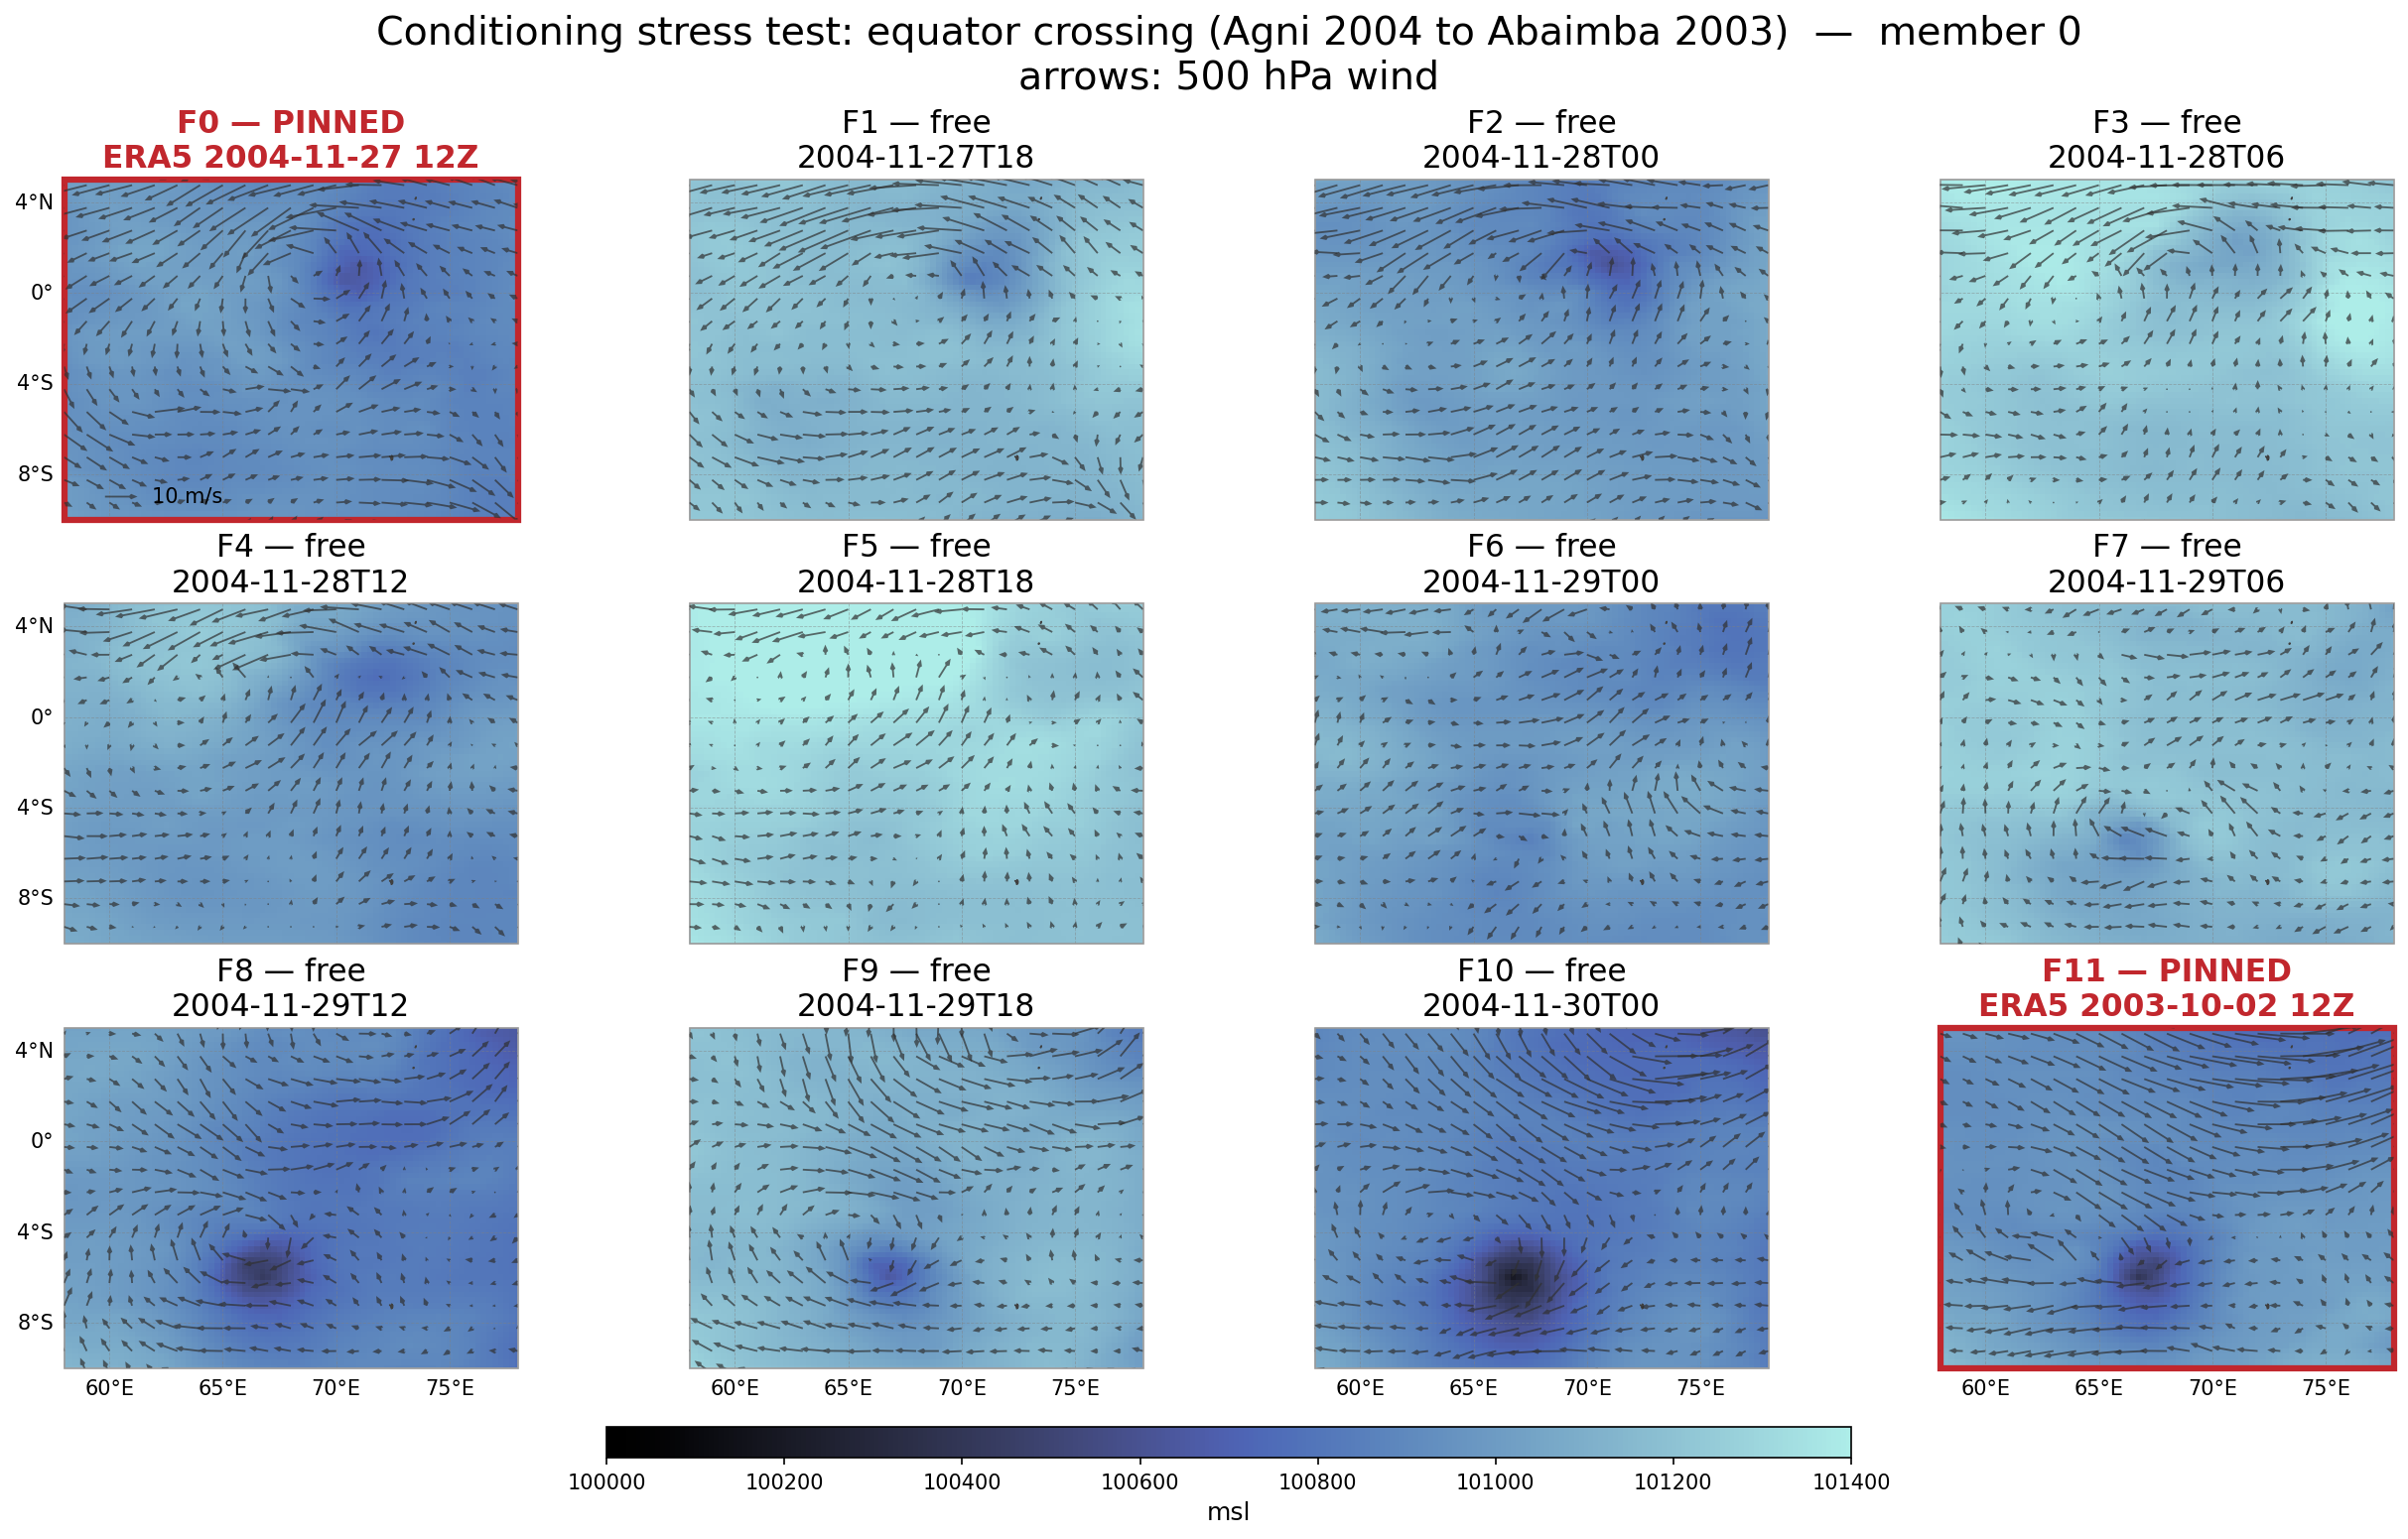
\includegraphics[width=\textwidth]{conditioning_stress_test.png}
\caption{Conditioning stress test: a both-end conditioned member generated from a pair of ERA5 analyses that no 66-hour trajectory connects. \textbf{All twelve panels are model output}; the red borders on F0 and F11 mark the two frames that were pinned and name the ERA5 state each was pinned to, rather than indicating panels taken from ERA5. Frame 0 is pinned to Cyclone Agni at 2004-11-27 12Z ($0.5^{\circ}$~N, $70.5^{\circ}$~E), an equatorial tropical low, and frame 11 to Tropical Storm Abaimba at 2003-10-02 12Z ($5.8^{\circ}$~S, $67.0^{\circ}$~E), located $\sim$790~km across the equator in the Southern Hemisphere. Shading shows MSLP on a common scale, arrows denote 500~hPa wind, and the regional domain is fixed at $58^{\circ}$--$78^{\circ}$~E, $10^{\circ}$~S--$5^{\circ}$~N. The model satisfies both terminal constraints: the Northern Hemisphere low decays over F1--F4, no organized vortex exists at F5--F6, and a Southern Hemisphere vortex emerges at F7 and intensifies into the terminal constraint. This experiment evaluates conditioning admissibility rather than forecast skill. Deliberate contrivances visible in panel headers include: endpoints drawn from different years, AMIP sea surface temperature clocked to the interval start time (supplying late-November-2004 SSTs to frame 11 rather than October-2003 values), and timestamps advancing 6-hourly from start time (frame 11 slot is 2004-11-30 06Z while the pinned field is 2003-10-02 12Z). Main-text Figure~3c presents the corresponding both-end result for dynamically adjacent endpoints.}
\label{fig:conditioning_stress_test}
\end{figure}

% Figures S13-S15 are the ageostrophic-fraction diagnostic, one float per case,
% cited from D4. Each PNG is already a complete twelve-panel figure, so as with
% S6-S11 they are not composed further: merging cases into one float would
% duplicate the (a)-(l) panel letters. h/w = 0.78, matching ian_tc_tracks.png,
% so they take its 0.82\textwidth sizing.
%
% The axis ranges of all three are pinned in scripts/_shared/axis_limits.yaml
% (analysis `ageostrophic`, variable `uvz500`) rather than autoscaled, which is
% what licenses the caption's claim that the three figures may be compared
% directly. If any of these PNGs is ever re-rendered, that block must still be
% in force or the claim becomes false -- the aggregator warns at plot time when
% data exceeds a configured limit, so a silent change is not possible.
\begin{figure}
\centering
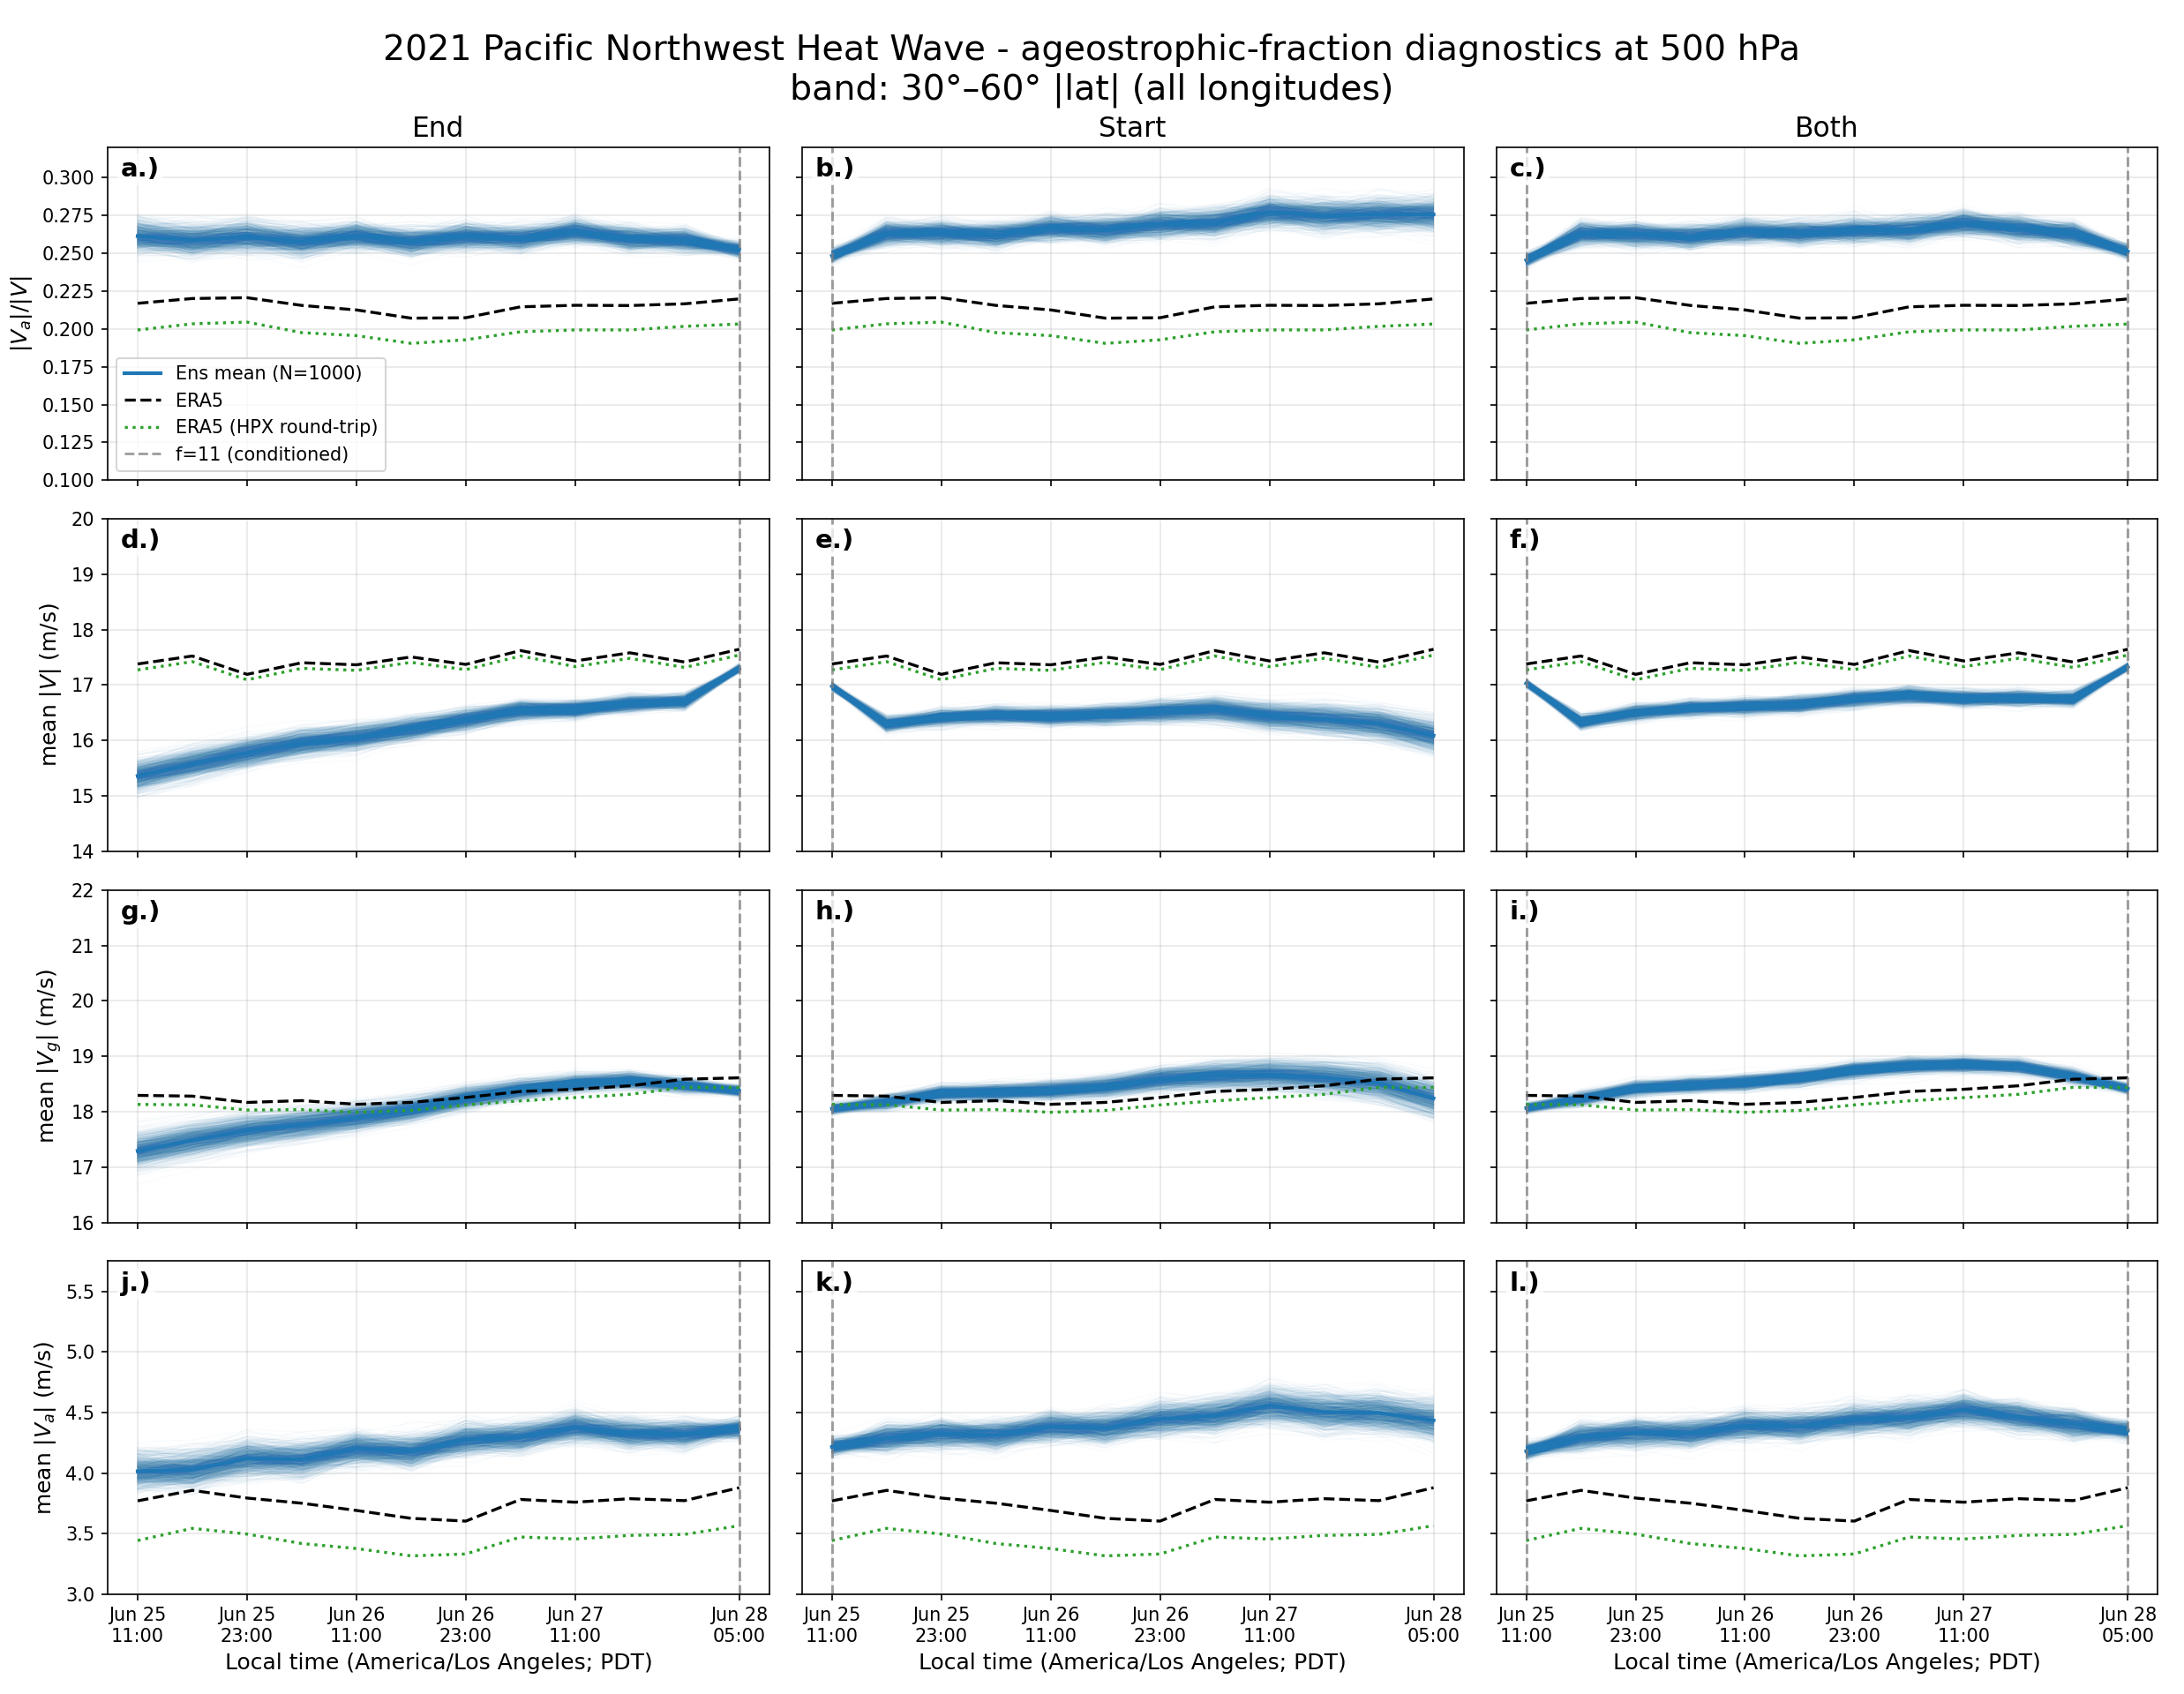
\includegraphics[width=0.82\textwidth]{ageostrophic_pnw_heatwave.png}
\caption{Ageostrophic diagnostics at 500~hPa for the 2021 Pacific Northwest heatwave ensembles across all three conditioning modes ($N = 1000$ each), as defined in Text~S5. Rows display the ageostrophic fraction $\langle |\mathbf{V}_{a}| \rangle / \langle |\mathbf{V}| \rangle$ (a--c) and $\cos\phi$-weighted mean speeds $\langle |\mathbf{V}| \rangle$ (d--f), $\langle |\mathbf{V}_{g}| \rangle$ (g--i), and $\langle |\mathbf{V}_{a}| \rangle$ (j--l); columns show end-, start-, and both-end conditioning. Individual ensemble members are shown in thin blue, ensemble means in bold blue, ERA5 in dashed black, and ERA5 passed through the HEALPix round-trip interpolation in dotted green. The green line, not the black, is the reference matching the ensemble's interpolation history (Text~S5); it lies below the black line, so regridding reduces the ageostrophic fraction rather than raising it. Gray dashed vertical lines mark each mode's pinned frames. Common axis ranges allow direct visual comparison across Figures~S13--S15. Mean speeds represent averages of vector magnitudes and are not additive across rows. What is measured is the ageostrophic fraction at one level, over one band, against one balance relation; it is not a general statement about balance in the generated fields.}
\label{fig:ageostrophic_pnw_heatwave}
\end{figure}

\begin{figure}
\centering
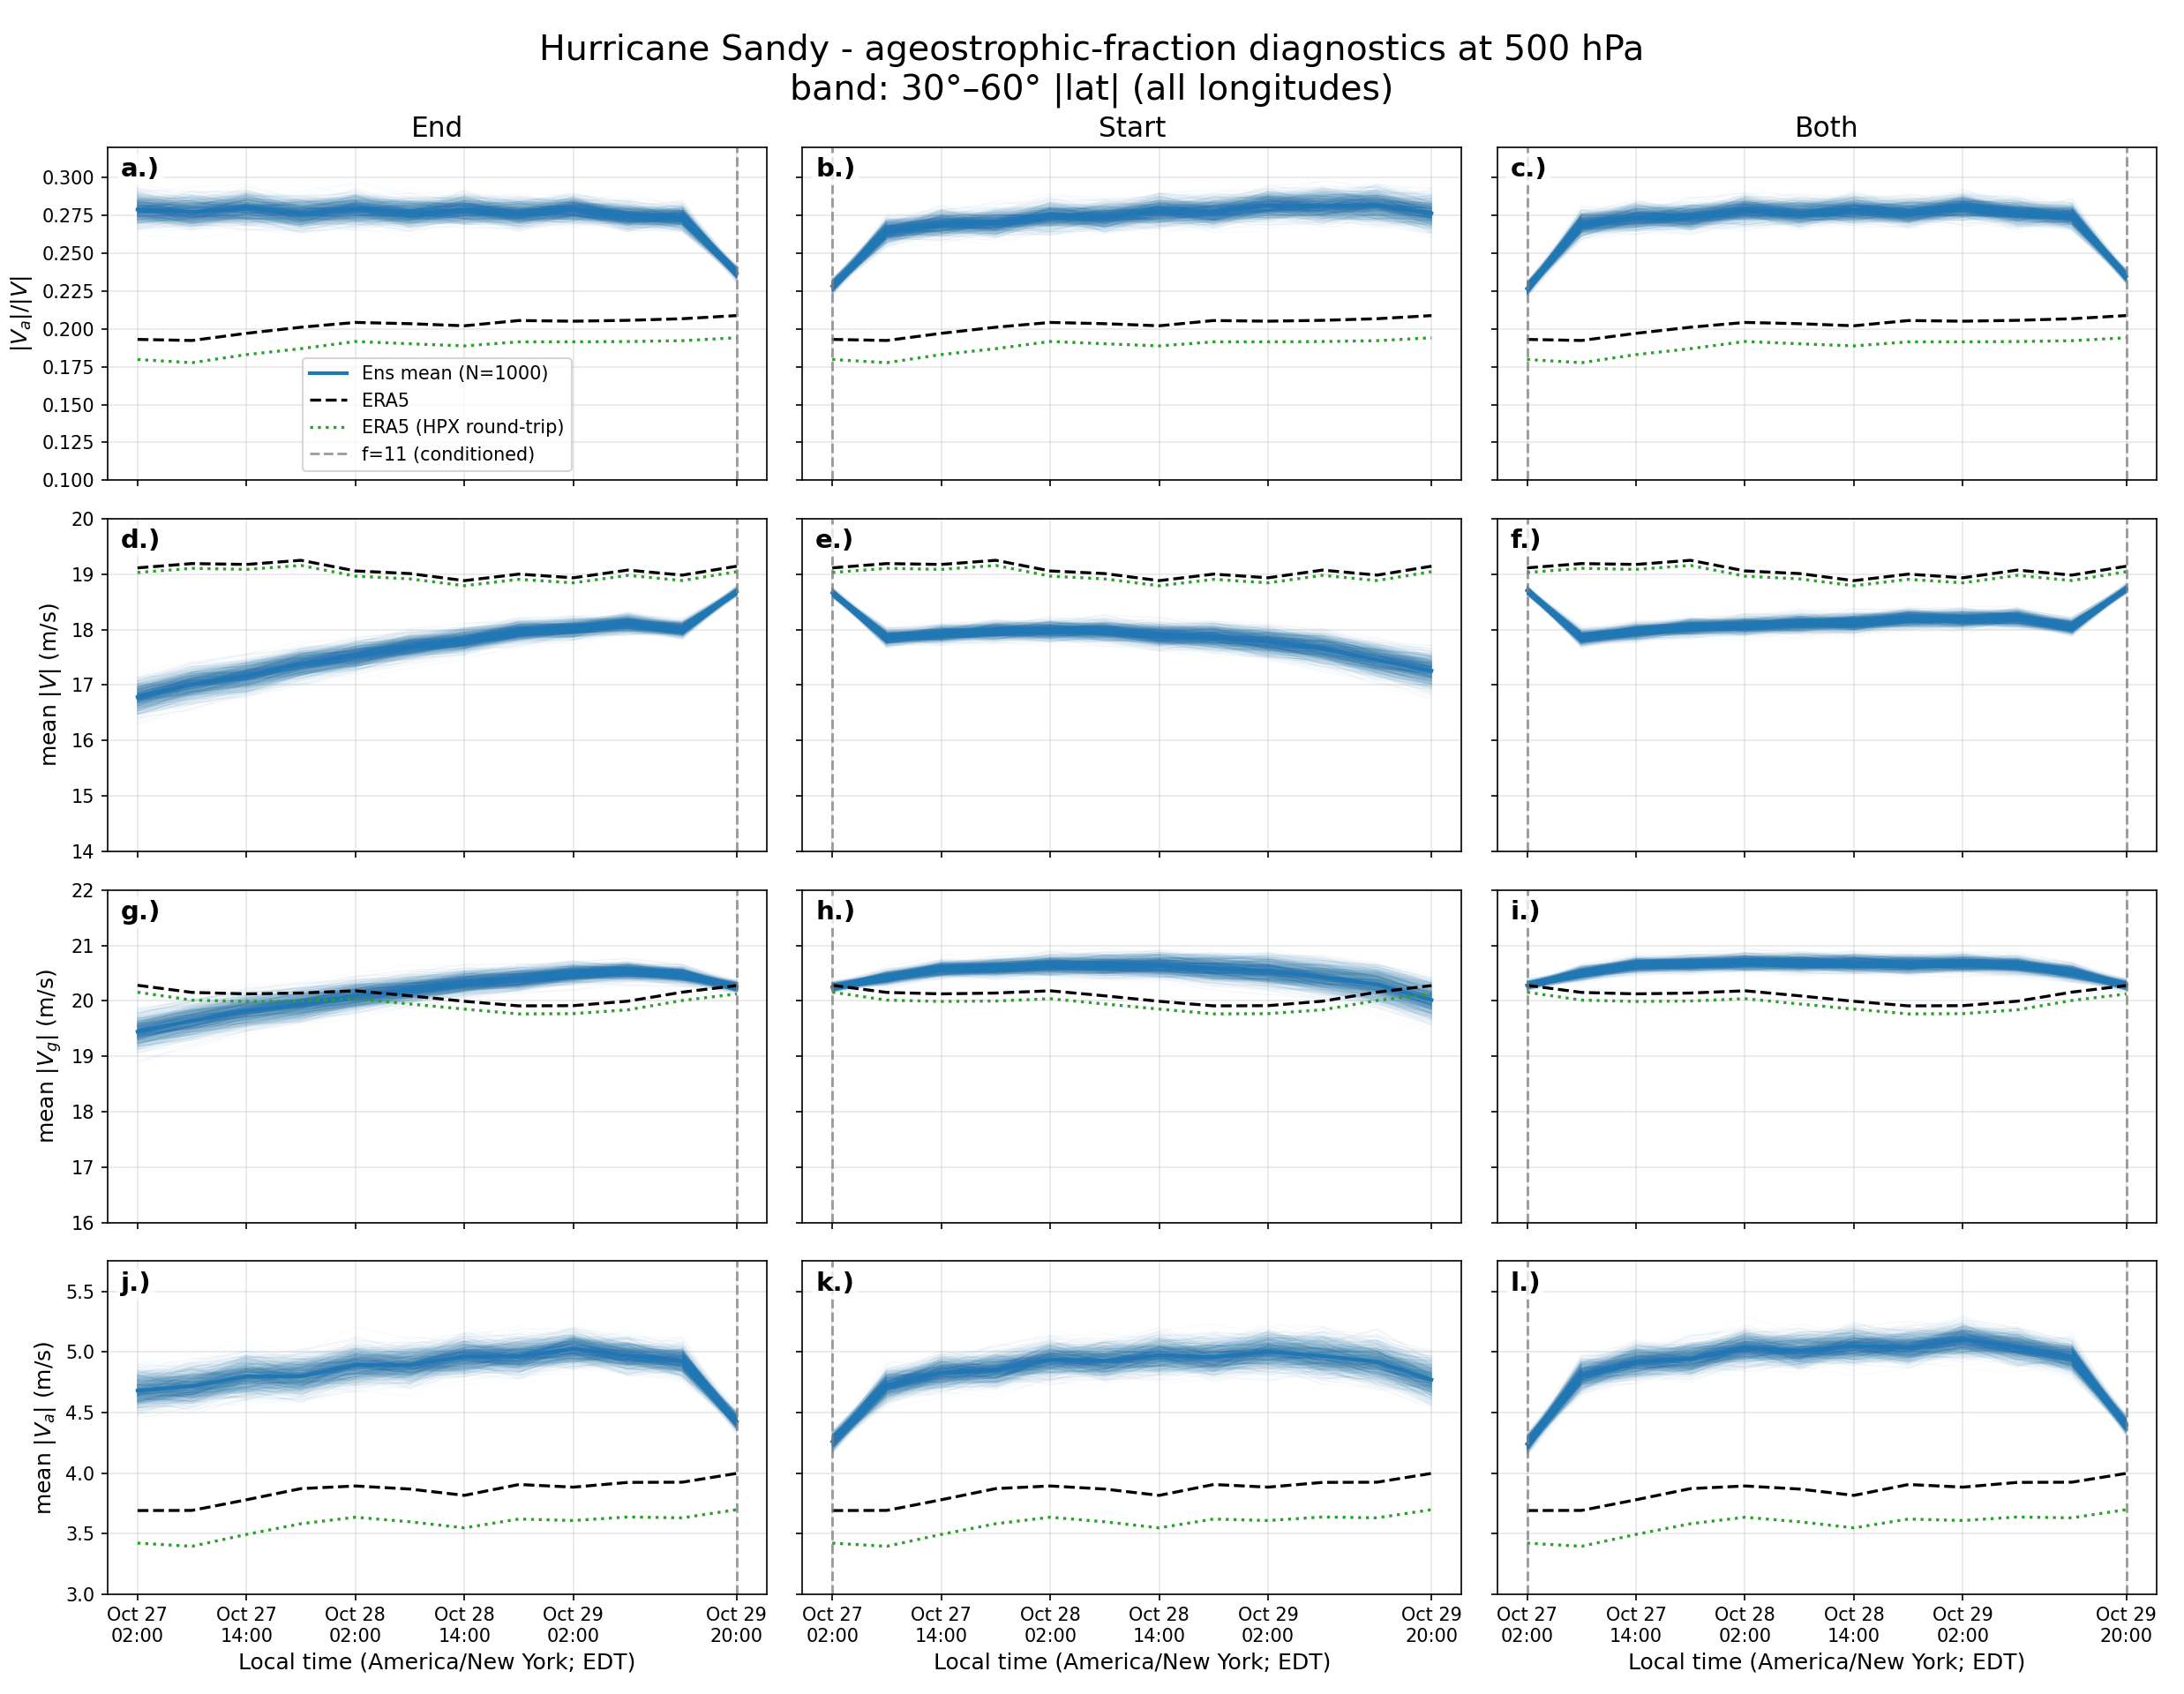
\includegraphics[width=0.82\textwidth]{ageostrophic_sandy.png}
\caption{As in Figure~S13, but for the Superstorm Sandy ensembles.}
\label{fig:ageostrophic_sandy}
\end{figure}

\begin{figure}
\centering
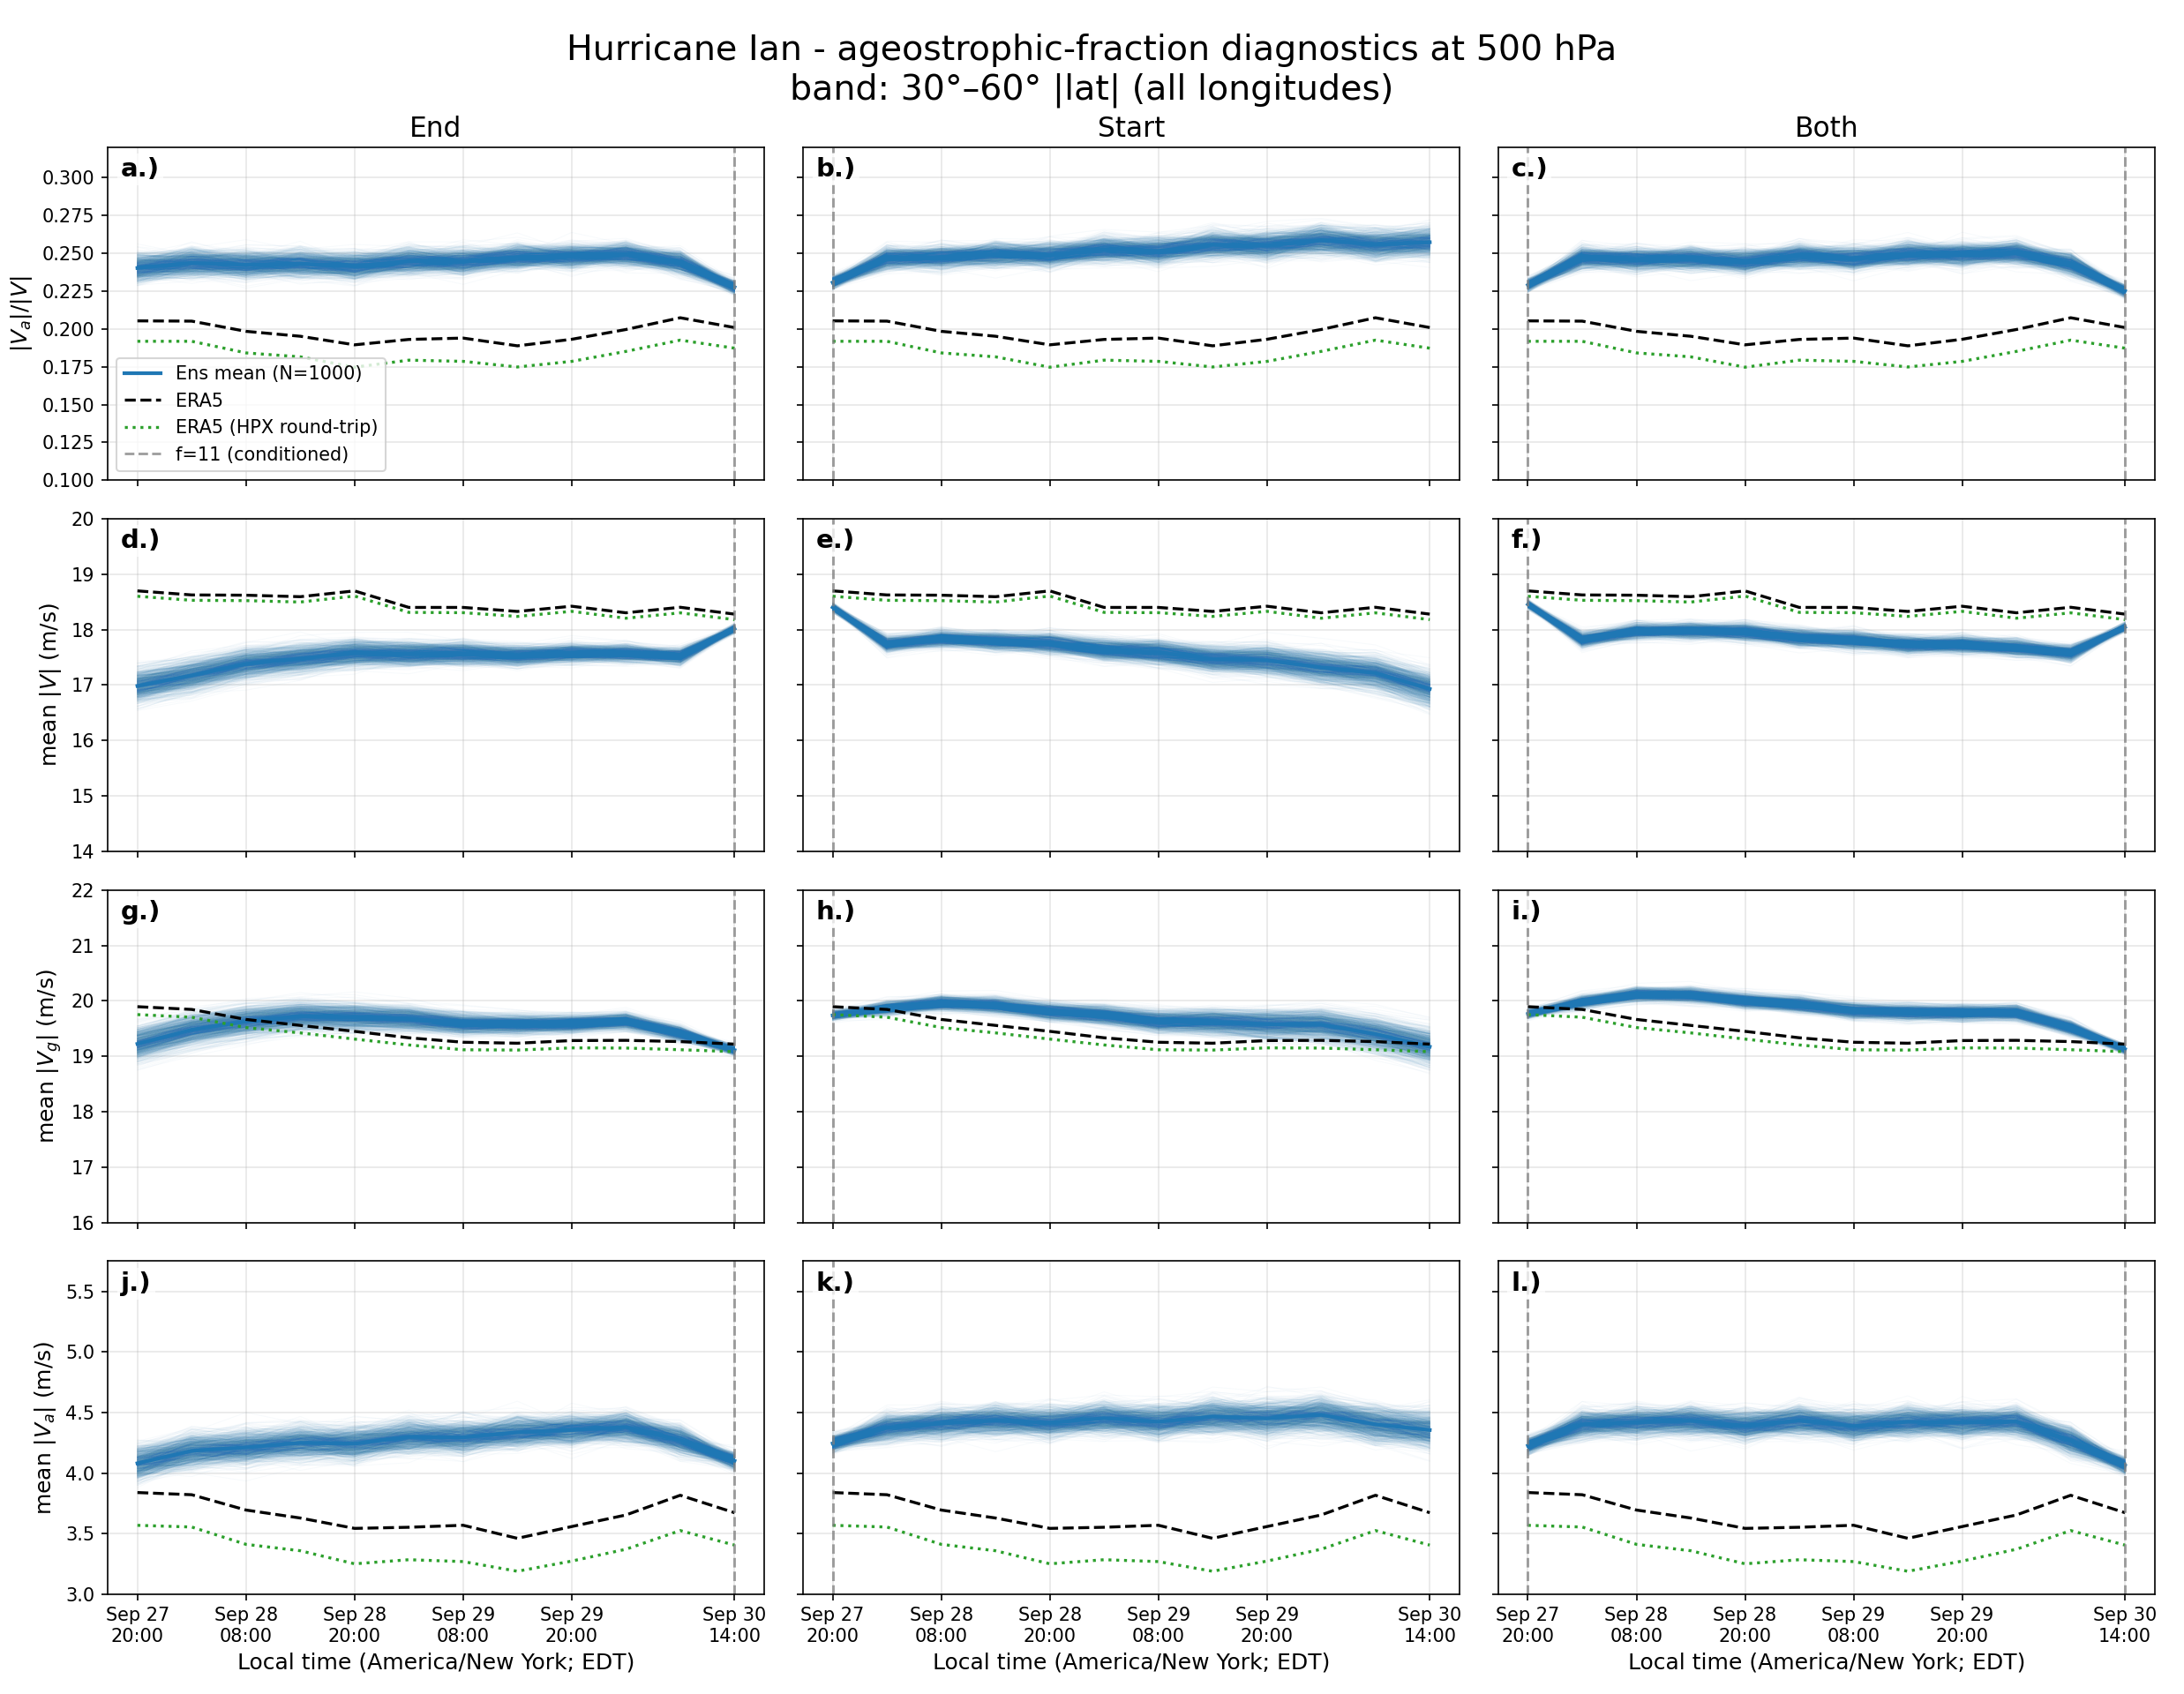
\includegraphics[width=0.82\textwidth]{ageostrophic_ian.png}
\caption{As in Figure~S13, but for the Hurricane Ian ensembles. The $30^{\circ}$--$60^{\circ}$~$|\phi|$ band excludes Ian's Florida-landfall latitudes by construction to preserve consistent cross-member spatial sampling, as detailed in Text~S5.}
\label{fig:ageostrophic_ian}
\end{figure}
